\documentclass[a4paper,11pt,oneside]{book}

\author{Vincenzo Maffione}
\title{Generic genetic algorithm on Intel SCC}
\date{\today}

%\usepackage{syntonly}
%\syntaxonly

\usepackage{lmodern} 

\usepackage{dsfont} % per i simboli degli insiemi di numeri (R,Z,Q,IR)
\usepackage{amssymb} % simboli matematici AMS
\usepackage{amsmath}

\usepackage{txfonts}

\hyphenation{pro-prie-t� in-di-vi-duo re-le-ga-re mo-del-lo mo-del-li o-pe-ra-zio-ni o-pe-ra-to-ri mo-du-lo ri-ve-la-to per-met-te-re rap-pre-sen-ta-zio-ne mo-del-liz-za-zio-ne ge-ne-ra-to o-biet-ti-vo li-ne-a-re no-no-stan-te po-si-ti-va e-la-bo-ra-zio-ne o-pe-ra-ti-vo sca-la-bi-li-t� i-ni-zia-liz-za-re in-di-vi-duo o-pe-ra-to-re va-lo-ri i-te-ra-zio-ni in-va-li-da-re pe-ri-fe-ri-che re-gi-stri ma-na-ge-ment e-si-ste pra-ti-ca va-ria-bi-li in-di-riz-zo o-pe-ra-zio-ne me-dian-te in-di-vi-duo sem-pli-ci-t� co-lo-ri ha-mil-to-nia-no que-sta in-clu-de-re ge-ne-tic}

\usepackage[italian]{babel}

%\usepackage{indentfirst} % indentazione nella prima riga di ogni capoverso

\setlength{\parindent}{0pt} % elimina l'indentazione sulla prima riga di ciascun capoverso


\usepackage[T1]{fontenc} % migliora la sillabazione di lingue non inglesi
\usepackage[latin1]{inputenc} %codifica per le lingue latine


% definizione dell'ambiente "abstract", per aggiungere il sommario
\usepackage{fancyhdr}
\newcommand{\fncyblank}{\fancyhf{}}
\newenvironment{abstract}%
{\cleardoublepage\fncyblank\null\vfill\begin{center}%
\bfseries\abstractname\end{center}}%
{\vfill\null}

\usepackage{graphicx}

\linespread{1.3}  % aumenta l'interlinea di un fattore 1.3


\begin{document}

%\maketitle

\begin{titlepage}
\pagestyle{empty}
\begingroup
% intestazione
\vspace*{-8.5\topskip}

\begin{figure}[!h]
\begin{center}

\includegraphics[scale=0.3]{logo_sssup}
\end{center}
\end{figure}

\vspace*{-0.5cm}

\begin{center}
        \large{\bf\expandafter\textsc {Scuola Superiore Sant'Anna}}\par 
		  \large{\bf\expandafter\textsc {Classe Accademica di Scienze Sperimentali}}\par
		  \large{\bf\expandafter\textsc {Settore di Ingegneria}}\par
        \vspace{0.5cm}
        \large{\bf\expandafter\textsc {Tesi di Licenza}}
\end{center}



% Titolo
\vspace{1.5cm}
\begin{center}
        {\LARGE\bf\textit{Algoritmo genetico parallelo sul Single-Chip Cloud Computer}}
\end{center}

\vspace{1.5cm}



\begin{center}
\begin{tabular}{l p{3.3cm} r c}

\textsc{Relatore} & & \textsc{Il candidato} \\
&&\\
\dotfill&&\dotfill \\
Prof. \textit{Giuseppe Lipari} & &\textit{Vincenzo Maffione}\\
{\small Scuola Superiore Sant'Anna} & &\\
 & &  \\
\textsc{Tutor} & &  \\
 \dotfill&&\\
Prof. \textit{Paolo Ancilotti} && \\
{\small Scuola Superiore Sant'Anna} && \\
 & & \\

\end{tabular}
\end{center}

\vspace{0cm}


\begin{center}
Anno Accademico 2010-2011
\end{center}
\par
\vfill\par 
\clearpage
\endgroup
  

\end{titlepage}

\newpage                                
\clearpage{\pagestyle{empty}\cleardoublepage}






\newpage\null\thispagestyle{empty}\newpage		%pagina bianca

\frontmatter					%Attiva numerazione romana perche' sei nell'intro


\begin{abstract}

Questo lavoro si pone come obiettivi:
\begin{enumerate}
	\item lo studio di un'architettura multicore basata sullo scambio di messaggi sviluppata da Intel, il Single Chip Cloud Computer.
	\item lo sviluppo su tale architettura, utilizzando il linguaggio C++, di un framework di ottimizzazione mono-obiettivo non vincolata basato su un \emph{algoritmo genetico parallelo}, ai fini di sperimentare il paradigma di programmazione a scambio di messaggi
\end{enumerate}

Le simulazioni effettuate evidenziano un graduale miglioramento dei risultati dell'ottimizzazione all'aumentare delle unit� di calcolo impiegate.

\end{abstract}


\newpage\null\thispagestyle{empty}\newpage		%pagina bianca


\tableofcontents
\listoffigures

\mainmatter					%Disattiva numerazione romana


\chapter{Introduzione ed obiettivi}

\section{Nuove tendenze architetturali}

La spinta verso il continuo aumento delle prestazioni dei processori che da sempre caratterizza la storia dei calcolatori elettronici ha portato negli ultimi anni allo sviluppo di nuovi modelli architetturali, basati sull'impiego di pi� unit� di elaborazione (CPU). Ne costituiscono un esempio i comuni PC dotati di processore multi-core o le architetture SMP (\emph{Symmetric Multi-Processing}), che sono al giorno d'oggi facilmente accessibili sul mercato.

\vspace{0.5cm}

La necessit� di dirigersi verso architetture multielaboratore � dettata da limiti e difficolt� di carattere tecnologico, che rendono molto complicato oppure sconveniente l'aumento della frequenza di lavoro dei chip al fine di incrementare le prestazioni e/o migliorare dell'efficienza energetica.

Aumentare la frequenza di lavoro significa infatti incrementare la potenza termica generata dal chip durante il suo normale funzionamento, con conseguente necessit� di dissipare il calore nell'ambiente.
Il problema pu� essere affrontato efficacemente riducendo progressivamente le dimensioni dei transistor di cui i chip sono costituiti. Si parla in questo senso di ottimizzare il \emph{processo produttivo}.

\vspace{0.5cm}

Sfortunatamente non � possibile ridurre indefinitivamente le dimensioni dei transistor, a causa del progressivo intensificarsi di effetti fisici indesiderati.

L'alternativa all'aumento della frequenza di lavoro (\emph{frequency scaling}), adottata da tutti i produttori, � quindi lo sviluppo di processori costituiti da pi� CPU.

Da osservare che l'aumento delle prestazioni ed il miglioramento dell'efficienza energetica � dovuto anche allo sviluppo di microarchitetture\footnote{Per \emph{microarchitettura} di un processore si intende lo schema logico espresso in termini di blocchi funzionali che descrive il funzionamento del processore stesso.} sempre pi� avanzate e ottimizzate. Ad esempio la tecnica dell'esecuzione fuori ordine (\emph{out-of-order execution}) sfrutta l'\emph{instruction-level parallelism} per raggiungere prestazioni pi� elevate. Un'altra tecnica � il cosiddetto \emph{simultaneous multi-threading}, che permette di eseguire pi� thread in parallelo su una stessa unit� di elaborazione.

\vspace{0.5cm}

Esistono vari modi con cui pi� CPU in uno stesso sistema di elaborazione possono comunicare tra loro, ed esistono anche diversi schemi con cui essi possono condividere risorse quali banchi di memoria RAM o memorie cache.

A titolo di esempio, i comuni processori \emph{dual-core} sono costituiti da due unit� di elaborazione che condividono la memoria centrale e tutte le risorse accessibili nel sistema. I due core possono condividere anche uno o pi� livelli di memoria cache.

Un processore dual-core di questo tipo � un esempio di architettura a memoria comune (\emph{shared memory}), in quanto la memoria centrale nella quale il sistema operativo ed i programmi applicativi risiedono durante il funzionamento del sistema � condivisa tra le due unit� di elaborazione.

Esistono sul mercato architetture multi-core a memoria comune con quattro, sei o otto unit� di elaborazione.

\vspace{0.5cm}

Nonostante l'architettura a memoria comune sia attualmente molto utilizzata, essa si � dimostrata poco scalabile nel momento in cui il numero dei processori aumenta ulteriormente, perch� tutte le unit� di elaborazione devono condividere l'unit� di comunicazione con la memoria centrale, il bus di memoria. Infatti, poich� il bus di memoria � utilizzabile da un core alla volta, all'aumentare del numero dei processori aumenta il tempo medio di attesa per l'accesso alla memoria.

Un utilizzo pi� intensivo del caching allevia questo problema, ma allo stesso tempo amplifica il problema della coerenza della cache (\emph{cache coerency}), che deve essere gestito al fine di garantire l'integrit� della memoria, e conseguentemente la correttezza delle elaborazioni effettuate.

Il costo del mantenimento della coerenza della cache, che si pu� ottenere ad esempio mediante l'utilizzo di tecniche di \emph{snooping} o di \emph{snarfing}, diventa progressivamente sempre pi� pesante all'aumentare del numero di core.

\vspace{0.5cm}

Per questi motivi, allo scopo incrementare ulteriormente il numero di unit� di elaborazione incorrendo il meno possibile in problemi di scalabilit�, sono stati sviluppati sistemi di elaborazione basati sull'architettura a memoria distribuita (\emph{distribuited memory}), nella quale ogni unit� di elaborazione dispone della propria memoria centrale. Non condividendo un'unica memoria centrale, le unit� di elaborazione devono comunicare scambiando messaggi mediante una apposita rete di comunicazione.
Per questo motivo le architetture a memoria distribuita vengono anche chiamate architetture \emph{a scambio di messaggi} (\emph{message passing}).

Se un'architettura a memoria distribuita viene realizzata su un singolo chip, si parla di \emph{Network-on-Chip} (NoC).

\vspace{0.5cm}

Il Single Chip Cloud Computer (per brevit� SCC) presentato da Intel nel 2010, oggetto di questo lavoro, � un esempio di Network-on-Chip.



\section{Obiettivi della tesi}
Questo lavoro si divide in due parti, che perseguono rispettivamente due obiettivi.

\vspace{0.5 cm}

Il primo obiettivo � quello di studiare l'architettura hardware dell'Intel Single Chip Cloud Computer ed il relativo software di supporto per il programmatore.
In modo particolare si studier� il funzionamento della libreria RCCE, disponibile al programmatore, ed il relativo paradigma di programmazione a cui bisogna attenersi.
L'interesse per un processore multicore a memoria distribuita che fornisce supporto per il message passing, quale � l'SCC, nasce dalle considerazioni fatte nella
sezione precedente.

\vspace{0.5 cm}

Il secondo obiettivo � quello di mettere in pratica gli strumenti e le metodologie apprese nella prima parte del lavoro per sviluppare una applicazione parallela
che sfrutti il pi� possibile le potenzialit� dell'SCC. A questo fine si � scelto di implementare un framework di ottimizzazione mono-obiettivo e non vincolato
basato su un \emph{algoritmo genetico parallelo}.




\chapter{Architettura dell'SCC}

\section{Introduzione all'SCC}
Il Single Chip Cloud Computer (SCC) � un microprocessore sperimentale creato nei laboratori Intel, ed alla data attuale � il processore che contiene il pi� alto numero di core (48) conformi alla Intel Architecture (IA) mai integrati su un singolo chip.

Nel settore dei supercomputer esistono da anni sistemi costituiti da centinaia o anche migliaia di core, ma in questi ultimi le singole unit� di elaborazione implementano un instruction set molto limitato, non paragonabile alla complissit� della Intel Architecture. In questo senso, l'SCC rappresenta un passo in avanti nel settore, in quanto la disponibilit� di un instruction set complesso permette l'utilizzo di un sistema operativo moderno completo.

L'SCC incorpora diverse tecnologie destinate ad essere impiegate su processori multi-core con un numero di core anche superiore alle 100 unit�, come ad esempio la tecnologia che realizza il network-on-chip, le tecnologie avanzate di gestione dell'alimentazione o il supporto per il message passing.

La nuova architettura multicore comprende alcune innovazioni che favoriscono la scalabilit� in termini di efficienza energetica: tra queste, un miglior meccanismo di comunicazione core-to-core e tecniche software che consentono di configurare dinamicamente tensione e frequenza di lavoro regolando consumi di potenza tra i 25W ed i 125W.

La piattaforma rappresenta l'ultimo risultato raggiunto dal progetto Intel \emph{Tera-scale Computing Research Program}. La ricerca � stata co-promossa dai laboratori Intel a Bangalore (India), i laboratori Intel a Braunschweig (Germania) e ricercatori dei laboratori Intel negli Stati Uniti.

Il nome Single-chip Cloud Computer riflette il fatto che l'architettura ricorda molto da vicino un cluster scalabile di computer (una \emph{nuvola} di computer), con la peculiarit� di essere integrato su un singolo wafer di silicio.

A grandi linee, il sistema comprende:
\begin{enumerate}
	\item 24 \emph{tiles} (ossia mattonelle) che compongono il cluster: ogni tiles contiene due core IA
	\item Una rete mesh composta da 24 router con picco di banda sul taglio pari a 256 GB/s
	\item 4 DDR3 memory controllers integrati
	\item supporto hardware per lo scambio dei messaggi
\end{enumerate}

\vspace{0.5cm}

Ogni core pu� caricare il proprio sistema operativo, comprensivo di stack di rete, e agire esattamente come agirebbe il nodo di una tradizionale rete di calcolatori a commutazione di pacchetto.

Uno degli aspetti pi� importanti della rete di comunicazione dell'SCC � che fornisce supporto a dei modelli di programmazione basati sullo scambio di messaggi che si sono dimostrati essere adatti per cluster composti da migliaia di processori.

Bench� ogni core abbia due livelli di cache, non viene fornito alcun supporto per la cache coherency, in modo da rendere pi� semplice l'architettura, ridurre i consumi, ed incoraggiare la ricerca sul calcolo distribuito on-chip basato su sistemi a memoria distribuita.

\vspace{0.5cm}
Un altro aspetto caratterizzante l'architettura � l'attenzione alla gestione dei consumi. Le applicazioni hanno la possibilit� di attivare/disattivare ogni core e regolare le performance in ogni istante, rendendo possibile la minimizzazione dei consumi, pur garantendo le prestazioni necessarie.

\'E possibile regolare regolare la tensione di alimentazione e la frequenza di lavoro sia della mesh che di alcuni sottoinsiemi di core. Ogni tile ha la propria frequenza di lavoro, e gruppi di 4 tiles possono funzionare ognuno con la propria tensione di alimentazione.


\section{Architettura}

Uno schema a blocchi dell'SCC � riportato in figura \ref{fig:SCC}.

\begin{figure}[bt]
\centering
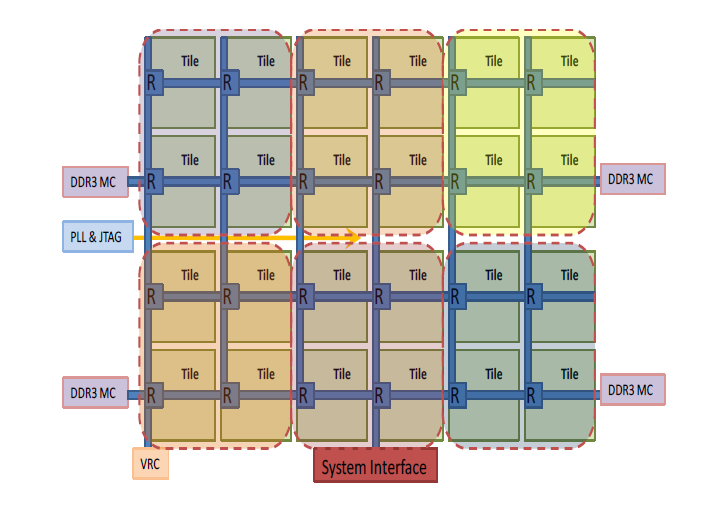
\includegraphics[scale = 0.45]{SCCBlockDiagram.png}
\caption{ Schema a blocchi dell'SCC }
\label{fig:SCC}
\end{figure}

I 48 core IA presenti nell'SCC sono microprocessori della famiglia P54C, uscita sul mercato nel 1994. Il processore P54C � relativamente semplice (rispetto ai core attuali): � dotato di due pipeline a 5 stadi, istruzioni floating-point, controllore avanzato delle interruzioni APIC, ma non ha un motore di esecuzione fuori ordine e non implementa le estensioni MMX.

I 48 core sono piazzati in una formazione a mattonelle (\emph{tiles}), con due core per ogni mattonella.

Le \emph{tiles} sono disposte in modo tale da formare una griglia bidimensionale (2D mesh) di dimensioni 6x4. Le comunicazioni avvengono per mezzo di
appositi router presenti all'interno di ogni tile.

I quattro memory controller integrati sul chip permettono di indirizzare fino ad un massimo di 64GB di memoria.
Pi� precisamente, ogni memory controller pu� indirizzare 2 banchi di memoria DIMM\footnote{\emph{dual in-line memory module} }, ognuno conentente 8GB di memoria.

Sono inoltre presenti, come supporto hardware allo scambio di messaggi, dei banchi di SRAM locali ad ogni tile.
Questo nuovo tipo di memoria, unito ad una nuova istruzione per la gestione della cache L1 interna al microprocessore P54C, facilitano la gestione
della memoria dell'SCC.

Il \emph{voltage regulator controller} (VRC) permette a qualsiasi core o l'interfaccia di sistema (SIF) di regolare la tensione di alimentazione in una qualsiasi delle regioni
tratteggiate mostrate in figura \ref{fig:SCC}, oltre alla tensione di alimentazione dell'intera griglia di router.
Questo metodo consente alle applciazioni un controllo totale del consumo di potenza.

L'interfaccia esterna di sistema, o SIF (\emph{system interface controller}) permette di mettere in comunicazione un router di bordo nella
rete mesh con l'esterno (precisamente, con un FPGA la cui funzione � descritta qui di seguito).

\vspace{0.5cm}

La piattaforma di sviluppo su cui il processore SCC � montato � costituita inoltre da un FPGA ed un \emph{board management microcontroller} (BMC).

L'FPGA fa le veci di un \emph{chipset}, fornendo tra le altre cose interfacce ethernet, interfacce SATA, 
un controllore globale delle interruzioni e registri contatori su cui � possibile fare incrementi in maniera atomica.

Da un punto di vista operativo l'SCC � controllato da un \emph{board management microcontroller} (BMC) che inizializza ed arresta le funzionalit� critiche
della piattaforma, e che si interfaccia, tramite PCI-Express, ad un comune PC che agisce da \emph{Management Console} (MCPC).

Tramite l'MCPC � dunque possibile caricare su ogni core un sistema operativo basato sul kernel Linux e caricare sui vari core una applicazione.

\begin{figure}[bt]
\centering
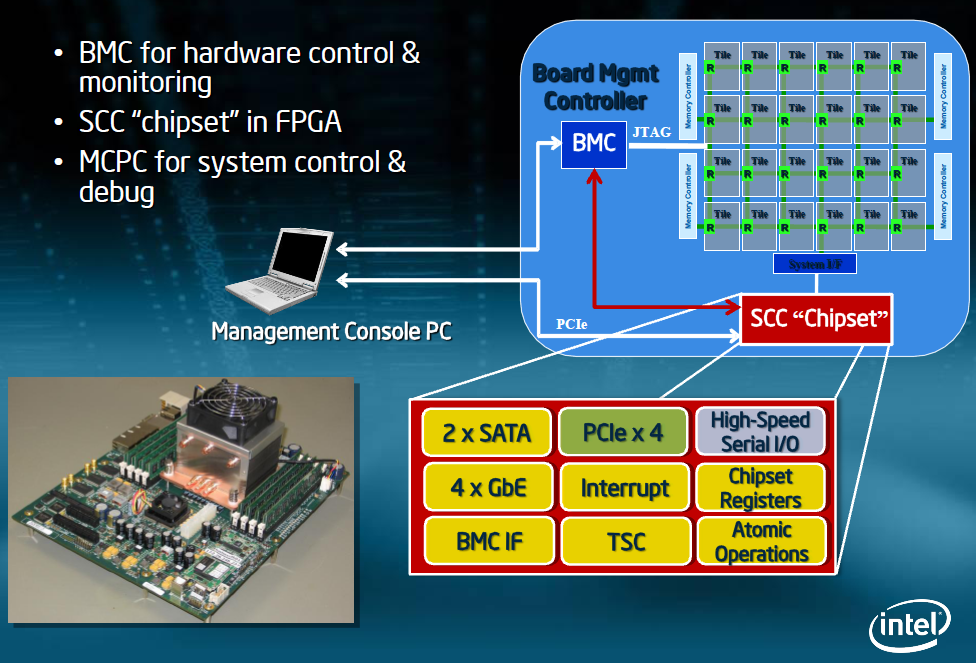
\includegraphics[scale = 0.45]{RockyLake.png}
\caption{ Piattaforma di sviluppo dell'SCC }
\label{fig:RockyLake}
\end{figure}

La piattaforma di ricerca � rappresentata in figura \ref{fig:RockyLake}.

\section{Descrizione del tile}
Ogni tile � composto dai seguenti elementi:
\begin{enumerate}
	\item Due IA core PC54C, con associati una cache L1 interna ed una cache L2 esterna
	\item Un crossbar router a 5 porte, che interfaccia il tile con la mesh e quindi con gli altri core
	\item Un generatore di traffico (TG) per testare la mesh, non accessibile via software,
	\item Una \emph{mes interface unit} (MIU) che gestisce tutti gli accessi alla memoria e le operazioni di scambio dei messaggi. Si noti che
		  la MIU � l'unica interfaccia che i due core interni al tile hanno con il router, e quindi con l'esterno. Allo stesso modo, i router costituiscono
		  l'unica interfaccia tra i vari tiles.
	\item Delle \emph{memory lookup table} (LUT) che permettono la traduzione degli indirizzi fisici di un core in indirizzi di sistema (ossia
		  indirizzi globali nell'SCC)
	\item Un message-passing buffer, che supporta lo scambio di messaggi.
	\item Ciruciterie per la generazione del clock e circuiterie di sincronizzazione per porre in comunicazione porzioni di circuiti che lavorano a
		  frequenze differenti (GCU e CCF)
\end{enumerate}

\begin{figure}[bt]
\centering
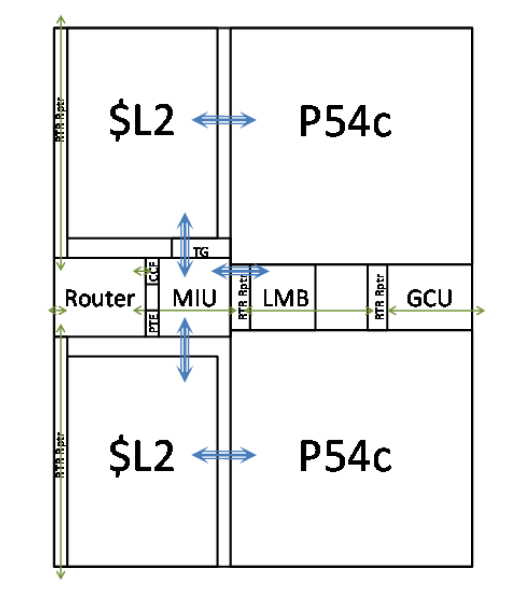
\includegraphics[scale = 0.45]{Tile.png}
\caption{ Schema a blocchi di un tile }
\label{fig:tile}
\end{figure}

Lo schema a blocchi di un tile � riportato in figura \ref{fig:tile}.

\section{ Descrizione funzionale dei componenti dell'SCC}

\subsection{Message passing buffer (MPB)}
In aggiunta alle tradizionali memorie cache, ogni tile � fornito di un buffer locale, il \emph{message passing buffer}, capace di operazioni
veloci di lettura/scrittura.
Questo buffer, grande 16KB, fornisce l'equivalente di 512 linee di memoria cache da 32 bytes.
Tutti i core e la SIF possono scrivere o leggere in uno qualasiasi degli MPB.
Sebbene l'MPB possa essere usato in qualsiasi modo, il suo principale utilizzo riguarda il meccanismo per lo scambio di messaggi, come verr� illustrato nel seguito.

\subsection{ Core P54C }
Il core, come gi� accennato, � un Pentium PC54. Il design originale � stato tuttavia leggermente alterato per aumentare fino a 16KB le dimensioni
della data cache e della instruction cache di primo livello (la singola linea ha dimensione pari a 32 bytes).
Le cache sono di tipo 4-way set associative con politica di rimpiazzo pseudo-LRU. In pi�, l'originale interfaccia tra bus di sistema e controllore della cache (M-unit)
� stata integrata all'interno del core.

L'instruction set del P54C � stato esteso con una nuova istruzione (\texttt{CL1INVMB}) ed un nuovo tipo di memoria (MPBT, ossia \emph{message passing buffer type}) 
allo scopo di facilitare il meccanismo di scambio dei messaggi.

L'istruzione \texttt{CL1INVMB} � stata aggiunta per invalidare tutte le linee della cache L1 che contengono dati di tipo MPBT.
A questo scopo la cache L1 � stata estesa aggiungendo ad ogni linea un bit che specifica se la stessa contiene dati di tipo MPBT.
Questo bit viene settato quando la linea di cache viene caricata con un dato di tipo MPBT. Per stabilire se un dato sia o meno di
tipo MPBT, bisogna considerare l'entrata della tabella della pagine relativamente alla pagina che contiene il dato. Questa entrata, oltre che in memoria virtuale,
� presente anche nel TLB (\emph{Translation lookaside buffers}). Il bit MPBT viene invece resettato quando il dato viene espulso dalla cache oppure quando
vengono eseguite le istruzioni \texttt{CL1INVMB}, \texttt{INVD} o \texttt{WBINVD}.
Di conseguenza, un nuovo bit � stato aggiunto in ogni entrata del TLB. Questo bit, presente in posizione 7 (� uno dei bit riservati, quindi precedentemente
inutilizzati), insieme al bit PCD (\emph{page cache disable}) ed al bit PWT (\emph{page write through}) determina il tipo di memoria della pagina in questione
(e quindi di un qualsiasi dato in essa presente). Le entrate delle tabelle delle pagine devono essere impostate dal sistema operativo.
Dati di questo tipo sono gestiti dalla cache L2 come non-cacheable: la M-unit del core assicura che i dati di tipo MPBT non siano mai caricati nella cache L2.
In altre parole per dati di tipo MPBT la cache L2 viene esempre bypassata.
Inoltre, i dati di tipo MPBT vengono trasferiti tra cache L1 e memoria condivisa (MPB oppure memoria condivisa off-chip) con la granularit� di 32 bytes.
Ci� non vale per dati non di tipo MPBT.

\begin{figure}[bt]
\centering
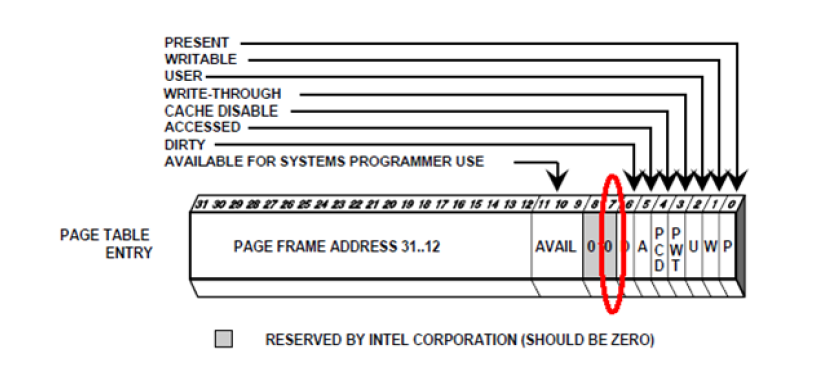
\includegraphics[scale = 0.45]{PageTableEntry.png}
\caption{ Entrata della tabella delle pagine del P54C }
\label{fig:pte}
\end{figure}

La struttura dell'entrata della tabella delle pagine � riportata in figura \ref{fig:pte};
Il tipo MPBT viene utilizzato principalmente per quella porzione di spazio di indirizzamento fisico che corrisponde all'MPB. In generale, il sistema
operativo pu� inizializzare la tabella delle pagine in modo dale che anche pagine fisiche di memoria off-chip siano etichettate come di tipo MPBT.
Poich� tuttavia l'SCC non implementa protocolli di cache coherency (snooping, snarfing, ecc.), conviene far s� che una qualsiasi porzione di 
memoria condivisa tra pi� core sia etichettata come di tipo MPBT, in modo tale da ottenere la coerenza della cache via software, nel modo
descritto di seguito.
Per accelerare il trasferimento di messaggi tra i core � stato inoltre aggiunto un \emph{write combine buffer} alla M-unit, che agisce sui dati di tipo MPBT.
Il write combine buffer trattiene nella M-unit i dati aggiornati da scrivere in memoria fino a quando non si riempie una intera linea di cache, oppure fino a quando non si tenta
di scrivere un'altra linea. Quando una di queste due situazioni si verifica, esso viene svuotato ed il comando di scrittura di una intera linea di cache viene
inviato in memoria.

\vspace{0.5cm}

Quando la \texttt{CL1INVMB} viene seguita, essa pone a zero tutti i bit MPBT della cache in un ciclo di clock.
Ogni linea di tipo MPBT viene invalidata. Se una linea da invalidare era stata modificata, il dato modificato non va ad
aggiornare la memoria, ma viene perso.
\'E responsabilit� del software assicurare che i dati di tipo MPBT presenti in cache non vadano persi.
Nel peggiore dei casi, si pu� eseguire l'istruzione \texttt{WBINVD}, la quale, prima di invalidare l'intera cache L1, si preoccupa di effettuare
l'operazione di \emph{write back}, ossia la propagazione verso l'esterno dei dati aggiornati (assicura la cache coerency).

\vspace{0.5cm}

Per quanto riguarda il message passing, l'istruzione \texttt{CL1INVMB} pu� essere usata per mantenere coerente la cache L1 (visto e considerato che la
cache L2 viene comunque bypassata) con il contenuto dalla memoria condivisa (MPB oppure memoria condivisa off-chip).
\'E sufficiente infatti eseguire la \texttt{CL1INVMB} prima di leggere dalla memoria condivisa per causare un read miss e dunque essere sicuri di leggere il contenuto attuale dell'MPB e non una copia non aggiornata dei dati in memoria condivisa (\emph{stale data}).
Analogamente, � sufficiente eseguire la \texttt{CL1INVMB} prima di scrivere nell'MPB per causare un write miss e forzare il P54C a emettere effettivamente una richiesta
di scrittura verso l'esterno. Infatti la politica in caso di write miss della cache L1 � \emph{no write allocate}. In altre parole, solo le
read miss comportano il caricamento del dato in cache. Se non eseguissimo la \texttt{CL1INVMB}, il dato da modificare con l'operazione di scrittura potrebbere
essere gi� presente in cache, ed in virt� della politica write-back la scrittura aggiornerebbe solamente la cache, non arrivando in memoria condivisa.


\subsection{ Cache L2 }
Ogni core ha la propria cache di secondo livello (256KB) con il controllore associato.
Durante un \emph{cache miss} di quest'ultima, il controllore invia l'indirizzo richiesto alla MIU, per la decodifica dell'indirizzo (si veda il paragrafo
dedicato alle lookup tables, o LUT) ed il successivo fetching in memoria.
Ogni core pu� avere in ogni istante solamente una richiesta pendente verso la memoria. Sar� quindi costretto ad attendere a causa di una \emph{read miss}
fino a quando i dati non arrivano dalla memoria.
In seguito ad una \emph{write miss}, invece, il core pu� continuare ad operare a patto che non si verifichi un altra write miss oppure una read miss.
All'arrivo del dato richiesto, il core pu� tornare ad operare normalmente.

Nonostante queste limitazioni, dovute all'impiego del P54C, il resto dell'hardware (la mesh ed il sistema della memoria) 
� capace di supportare pi� richieste pendenti.
La cache L2 � di tipo 4-way set associative con politica di rimpiazzo pseudo-LRU. Pu� essere usata solo in modalit� \emph{write-back} e non supporta la
modalit� \emph{write-allocate}.

Nell'SCC, le istruzioni \texttt{INVD} e \texttt{WBINVD} eseguite da un core non hanno alcun effetto sulla cache L2 del core stesso.


\subsection{Tabelle di lookup per la traduzione degli indirizzi}
Ogni core dispone di una \emph{lookup table} (LUT) che � formata da un insieme di registri di configurazione (che sono a loro volta mappati in memoria
tramite loro stessi). Questa tabella mappa gli indirizzi fisici del core nello spazio di indirizzi di sistema dell'SCC (indirizzi globali).
Una LUT contiene 256 entrate, una per ogni porzione dello spazio di indirizzamento fisico del processore, che � di 4GB (gli indirizzi del core sono su 32 bit).
Di conseguenza ogni entrata della LUT mappa 16MB dello spazio fisico di indirizzamento del processore.
Ogni entrata della LUT pu� puntare ad una qualsiasi locazione di memoria: le memoria privata del core (la RAM off-chip accedibile tramite i 4 memory controller),
il message passing buffer, i registri di configurazione del core, l'interfaccia di sistema (SIF) o il controllore dell'alimentazione.
Il LUT pu� essere programmato dalla Management Console per mezzo di scritture che attraverso la SIF. Normalmente, le sue entrate sono
inizializzate con una configurazione opportuna  durante il processo di bootstrap del sistema. Dopo il boot, una generica LUT pu� essere dinamicamente
modificata da qualsiasi core che sia capace di indirizzarla attraverso la propria LUT.
Quando si verifica una chache miss della cache L2, la MIU consulta la LUT per determinare dove la richiesta di memoria debba essere spedita.

\subsection{ Mesh Interface Unit (MIU) }
La Mesh Interface Unit (MIU) contiene i seguenti blocchi funzionali:
\begin{enumerate}
	\item Pacchettizzatore e depacchettizzatore
	\item Interprete dei comandi provenienti dall'esterno, decodificatore degli indirizzi
	\item Alcuni registri locali di configurazione
	\item Logica per il controllo di flusso a livello di collegamento (livello data link)
	\item Un arbitro per coordinare richieste diverse provenienti da agenti diversi
\end{enumerate}

Il pacchettizzatore/depacchettizzatore traduce i dati da/verso gli agenti alla/dalla mesh.

Pi� in dettaglio, al verificarsi di una cache miss L2, la MIU decodifica l'indirizzo del dato richiesto, utilizzando 
la LUT per tradurre l'indirizzo locale del core in un indirizzo di sistema. Dunque inserisce la richiesta in una coda
appropriata.
Ci sono tre code di richieste:
\begin{enumerate}
	\item Richieste per l'accesso al router, e quindi alla memoria off-chip.
	\item Accesso al message passing buffer
	\item Accesso ai registri locali di configurazione
\end{enumerate}

Per quanto riguarda il traffico proveniente dal router, la MIU � responsabile di dirottare i dati verso 
la destinazione locale appropriata. Il controllo di flusso a livello data link � gestito attraverso un
protocollo credit-based.

L'arbitro opera secondo una politica round robin.

\begin{figure}[bt]
\centering
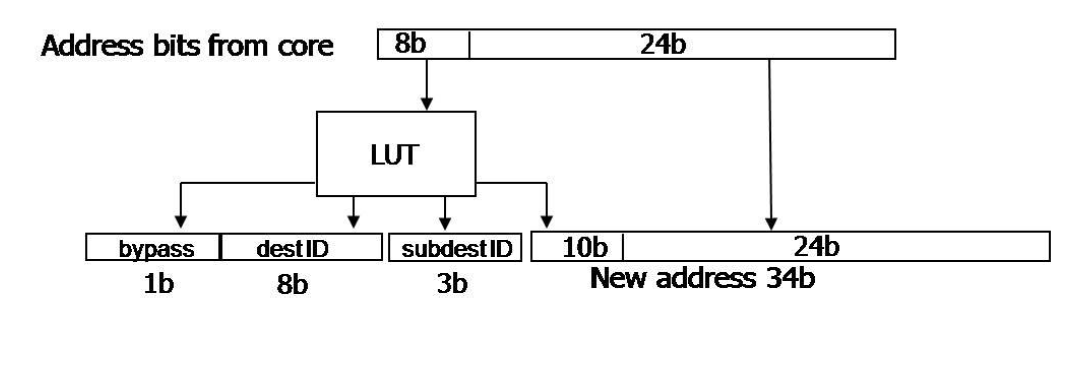
\includegraphics[scale = 0.45]{LUT.png}
\caption{ Schema di traduzione degli indirizzi }
\label{fig:LUT}
\end{figure}

Il core lavora con indirizzi fisici a 32-bit. Gli 8 bit pi� significativi sono usati direttamente come indice nella
LUT in concomitanza di una cache miss. Il LUT emette in uscita 22 bit: 10 bit di estensione per l'indirizzo di sistema, 8 bit di
\texttt{tileID}, 3 bit di \texttt{sub-destinationID} e un bit di \emph{bypass}.
Il campo \texttt{tileID} � un identificatore che specifica il tile destinazione della richiesta di accesso in memoria effettuata dal core.
Il campo \texttt{sub-destinationID}, che va interpretato in base al valore del campo \texttt{tileID}, specifica su quale porta del router destinatario il pacchetto inviato
dovr� essere rediretto e/o qual � il dispositivo destinatario: potrebbe trattarsi di un MPB, di un registro di configurazione, di un memory controller,
del VRC (voltage regulator controller) oppure dell'interfaccia di sistema (SIF).
L'indirizzo di sistema � dunque a 46-bit: il bit di bypass + 3 bit di \texttt{sub-destinationID}
+ 8 bit di \texttt{tileID} + 10 bit di estensione dell'indirizzo + i 24 bit meno significativi dell'indirizzo a 32-bit del core.

Il \texttt{sub-destinationID} definisce la porta dalla quale il pacchetto lascia il router (porta est, ovest, nord, sud).

Il tile specificato dal campo \texttt{tileID} (tile destinatario) riceve il pachetto inviato dal router e utilizzando il campo \texttt{sub-destinationID} (inviato anch'esso nel pacchetto)
decide quale destinazione prendere. Il bit di bypass specifica accessi locali all'MPB.

I 34 bit meno significativi dell'indirizzo di sistema tradotto vengono spediti al tile destinatario.

Il campo \texttt{tileID} � codificato in maniera tale da permettere ai router di effettuare il routing dei pacchetti in modo corretto.

\subsection{Registri di configurazione}
I registri di configurazione presenti in ciascun tile forniscono alle applicazioni la possibilit� di controllare i modi di operazione delle 
varie unit� hardware presenti nel tile stesso. Questi registri controllano l'abilitazione del reset locale, le impostazioni del clock locale, la configurazione
iniziale dei core, la gestione delle interruzioni e la configurazione della cache L2.
Ogni core, cache controller della L2 o unit� di gestione del clock ha un registro di configurazione dedicato che � accessibile in scrittura da qualsiasi altro core
e dalla SIF. In pi� sono presenti dei \emph{test-and-set register} per rendere possibili i protocolli di comunicazione (ad esempio un protocollo basato sullo
 scambio di messaggi) in ambito multi-processore.
Pi� in dettaglio, ogni core possiede il proprio test-and-set register. Il valore iniziale di tali registri � 1. Un core acquisice il lock leggendo un
test-and-set register ed ottenendo uno. Qualsiasi core (non necessariamente quello che ha acquisito il lock) pu� rilasciare il lock scrivendo un qualsiasi
valore nel test-and-set register. Per convenzione, all'atto del rilascio viene scritto il valore 0.

Al reset, i registri di configurazione sono settati con dei valori ben noti e sicuri.
Per modificare i registri di configurazione, � necessario seguire il paradigma read-modify-write sull'intero registro a 32 bit, per essere sicuri
che l'operazione avvenga correttamente (non sono supportati accessi a porzioni di bit inferiori a 32-bit).

Il registro di configurazione di un bit contiene anche i due bit di interrupt: il bit \texttt{INTR} che segnala le interruzioni mascherabili
ed il bit \texttt{NMI} che segnala le interruzioni non mascherabili. I due bit del registro sono connessi direttamente ai rispettivi pin di interrupt
del core.

\subsection{Voltage regulator controller}
Il \emph{Voltage regulator controller} (VRC) � gestito attraverso delle locazioni di memoria di sistema accessibili da un qualunque core
abbia mappato tali locazioni nella propria LUT.

Una scrittura in queste locazioni si traduce in un comando per il VRC, che viene spedito sulla mesh ed eseguito.
Il VRC accetta il comando, modifica la tensione di alimentazione, ed infine invia un riscontro al tile che ha generato
il comando, cosicch� quest'ultimo possa essere sicuro che il comando sia stato eseguito con successo.

In fase di inizializzazione del sistema, il VRC deve ricevere i comandi per fornire l'alimentazione ai tiles, in modo tale che questi possano essere resettati.
Successivamente, il VRC pu� ricevere richieste addizionali: togliere l'alimentazione ad un sottoinsieme di tiles, passare in
modalit� risparmio energetico, passare in modalit� alte prestazioni, etc. ).

\subsection{Rete mesh}
La rete mesh di cui l'SCC � dotato, � formata da 24 router che commutano pacchetti in una configurazione 6x4 (conforme alla formazione dei tiles). La
rete � dotata di una sua sorgente di alimentazione e di un suo generatore di clock, separati da quelli del resto del chip. Ci� permette di trovare
un compromesso ottimale tra consumi e prestazioni.

Il router utilizzato (RXB) � un router di nuova generazione pensato per le future strutture mesh bidimensionali da utilizzarsi per processori multicore
analoghi all'SCC. Le sue caratteristiche sono le seguenti:
\begin{enumerate}
	\item Larghezza dei collegamenti: 16 bit per la linea dati + 2 bit per segnali di controllo
	\item Frequenza: 2 Ghz
	\item Latenza: 4 cicli, includendo l'attraversamento del link
	\item Diverse classi di messaggi: una classe di messaggio per le richieste ed una classe di messaggi per e risposte
	\item Pi� canali virtuali (VC): 1 VC riservato per ogni classe di messaggi + 6 VC a disposizione per un totale di 8 VC
	\item Gestione dinamica dell'alimentazione: modalit� di sleep, controllo della tensione, clock gating\footnote{Il \emph{clock gating} � una tecnica di 
	      progetto di circuiti digitali in base alla quale si cerca di fornire il clock solo a quelle porzioni di circuito che in un dato istante
		  stanno effettivamente lavorando, riducendo cos� i consumi globali medi}, ecc..
\end{enumerate}

Gli agenti della mesh commuicano tra di loro tramite scambio di pacchetti. Un pacchetto corrisponde di uno o pi� \emph{flit} (fino 
ad un massimo di tre flit). Un pacchetto dati � composto da tre flit, con l'header nel primo flit, il corpo nel secondo e la coda nel terzo.
I flit di controllo (che non sono pacchetti contenenti dati utili) sono utilizzati per scambiare informazioni di controllo quali i crediti (utilizzati nel
protocollo di controllo di flusso).

Il controllo dell'errore viene effettuato end-to-end, principalemente attraverso l'uso di diversi bit di parit�, applicati alle informazioni di instradamento, 
alle informazioni di comando ed ai dati.

I percorsi seguiti dai pacchetti vengono instradati secondo una semplice politica x-y: un pacchetto si sposta prima orizzontalmente fino all'ascissa di
destinazione e successivamente si muove verticalmente.


\section{Gestione dinamica della frequenza di funzionamento e della tensione di alimentazione}
I core dell'SCC sono divisi in sei \emph{voltage island} (o \emph{voltage domain}), ognuna contenente una matrice 2x2 di tiles. Ogni isola ha dunque in totale
di otto P54C core.
Ciascuna isola possiede una propria sorgente di alimentazione. Il clock � invece fornito ad un livello pi� piccolo di granularit�, in modo che ogni tile possa
operare ad una sua propria frequenza. Le isole di tensione e di frequenza rendono possibile lo spegnimento o la riduzione dei consumi (e quindi delle 
prestazioni) di sottoinsiemi dell'SCC, in modo da minimizzare il consumo di energia.
La regolazione pu� avvenire sotto il controllo dell'applicazione che pu� impostare il livello di prestazione voluto in specifici
gruppi di tiles.

\vspace{0.5 cm}

Sono dunque possibili diversi paradigmi per il controllo delle performance. Ad esempio:
\begin{itemize}
	\item un core controlla tutti gli altri
	\item ogni core controlla s� stesso
	\item ogni core controlloa il quadrante in cui si trova
\end{itemize}

Come gi� accennato, la mesh ha un proprio generatore di clock e una propria sorgente di alimentazione, condivise da tutti i router nella griglia.
Per questo motivo, qualsiasi comunicazione tra un router e l'hardware all'interno del tile (o altre periferiche connesse all'SCC) richiedono 
dell'hardware di raccordo (level shifter e asynchronous clock transition): queste ultime funzionalit� sono fornite dall'unit� CCF (clock crossing FIFO).
I consumi della mesh possono dunque essere controllati indipendentemente da quelli dei core, e viceversa. Si pu� dunque pensare all'intera mesh come 
un'unico dominio di frequenza/tensione.



\chapter{Programmazione con l'SCC}

\section{Introduzione}
L'SCC fornisce strumenti di basso livello per supportare diversi paradigmi di programmazione. Il paradigma tipicamente utilizzato si
basa su una qualche forma di message passing. Come gi� accennato, i messaggi vengono trasferiti nel chip utilizzando i
message passing buffer (MPB). Come descritto nel capitolo precedente, l'SCC supporta diverse configurazioni della memoria off-chip (la RAM esterna
accedibile tramite i quattro memory controller), esponendo i registri di configurazione delle tabelle di lookup (LUT). In ogni istante, 
l'applicazione pu� modificare il modo in cui gli indirizzi fisici di un dato core vengono tradotti (mappati) in indirizzi di sistema.

Gli indirizzi fisici di ogni core possono essere mappati sugli indirizzi di sistema in modo tale da far s� che tutta, parte, o nessuna parte del loro spazio di
indirizzamento si riferisca ad una porzione di memoria condivisa tra determinati insiemi di core.

La suddivisione della memoria off-chip tra memoria privata a ciascun core e memoria condivisa tra gruppi di core � programmabile
in modo dinamico, in modo da rendere il sistema flessibile nel partizionare compiti tra i core.
La memoria condivisa pu� essere usata per scambiare dati fra i core, o per memorizzare dati (ad esempio la si potrebbe utilizzare per
implementare un database in-memory).
Pu� essere convieniente disabilitare il caching per la porzione di memoria condivisa, oppure gestire la coerenza della cache via software.

Tutti gli accessi di I/O sono rediretti sull'interfaccia di sistema (SIF) e dunque all'FPGA off-chip.

\vspace{0.5cm}

Come accennato nel capitolo precedente, le interruzioni vengono segnalate ad un determinato core settando e resettando un bit appropriato nel registro
di configurazione di quel core. Il software pu� generare interruzioni non mascherabili, interruzioni mascherabili oppure interruzioni
per la gestione del sistema (\emph{systema management interrupt}). Il modo in cui un core processa le interruzioni � configurato
nella Local Vector Table (LVT) del Local APIC di cui il P54C � dotato.

L'SCC dispone di diversi metodi di reset della logica dei core, a vari livelli di granularit�: a titolo di accenno, esiste l'\emph{hard reset}, il \emph{soft reset},
il \emph{direct single core reset} ed il \emph{direct single L2 cache reset}.

\vspace{0.5 cm}

In fase di inizializzazione della piattaforma su cui � montato l'SCC, su ogni core viene caricato un sistema operativo basato sul kernel di Linux.
Ogni core dispone della sua copia del sistema operativo, presente nella sua memoria privata. A livello operativo, i programmi applicativi con cui si vogliono
sperimentare le potenzialit� dell'SCC possono essere caricati sfruttando lo stack di rete attivo su tutti i core. Attraverso l'interfaccia di sistema (SIF)
vengono stabilite delle connessioni ssh tra l'MCPC ed i core, in modo da poter lanciare le applicazioni semplicemente eseguendo un comando remoto dall'MCPC.


\section{La libreria RCCE}
\label{sez:alloc}
Per utilizzare l'SCC allo scopo di effettuare ricerche sulle architetture a scambio di messaggi, � stata sviluppata la libreria RCCE, una libreria leggera
e di dimensioni contenute che implementa le funzionalit� minimali per consentire lo scambio di messaggi tra i core.
La libreria utilizza gli MPB presenti nei tiles (si ricordi che si tratta di memoria on-chip) per trasferire dati tra core differenti.

L'MBP � un'area di memoria condivisa, e dunque in teoria potrebbe essere utilizzata in un modo qualsiasi dalle applicazioni.
Poich� tuttavia ogni MPB � grande solo 16KB\footnote{si consideri inoltre che i 16KB sono dedicati complessivamente ad un tile, e quindi andrebbero
suddivisi tra i due core}, � conveniente utilizzarlo unicamente come buffer per lo scambio di messaggi. La dimensione dell'MPB �
infatti troppo piccola perch� esso possa essere utilizzato per memorizzare le strutture dati di un'applicazione di medie dimensioni.

RCCE � una libreria di basso livello, che era inizialmente stata concepita per lavorare sull'SCC senza il supporto del sistema operativo
(si parla di \emph{bare metal mode}). Di conseguenza, essa � stata sviluppata senza fare affidamento ai tipici servizi che un sistema operativo offre.

Solo successivamente � stato possibile effettuare il porting di Linux sull'SCC, e da quel momento in poi si � in generale preferito lavorare con Linux.

\vspace{0.5 cm}

Per questi motivi, le scelte di progetto effettuate per RCCE hanno comportato una notevole riduzione degli overhead. Innanzitutto, senza sistema operativo
non esiste il concetto di unit� di schedulazione, e dunque RCCE � pensata per eseguire una singola applicazione, senza necessit� di richiedere servizi al
sistema operativo portando il processore in modalit� sistema. Ci� non rende possibile effettuare comunicazioni asincrone, poich� un'implementazione
di queste ultime richiederebbe l'utilizzo di pi� thread. Di conseguenza le operazioni di invio e ricezione sono necessariamente bloccanti. Se da un lato
ci� costituisce una limitazione, dall'altro semplifica enormemente la gestione dei messaggi, dal momento che in ogni istante ci pu� essere solamente una 
comunicazione in attesa di completamento tra ogni coppia di core.
Ci� comporta che:
\begin{itemize}
	\item non ci sono code di messaggi
	\item sono sufficienti due variabili di sincronizzazione per ogni coppia di core comunicanti
	\item l'MPB pu� essere interamente dedicato al payload della comunicazione (al netto dello spazio necessario per le variabili di sincronizzazione)
\end{itemize}
Il modello di programmazione fornito da RCCE � molto semplice: si basa sul paradigma \emph{Single Program Multiple Data} (SPMD).
Di conseguenza, lo stesso eseguibile viene caricato su tutti i core. Nel codice sorgente, i costrutti condizionali possono essere utilizzati per far eseguire
parti di codice solo a determinate unit� di esecuzione (ad ogni unit� di esecuzione � associato un identificatore, utilizzabile nel codice sorgente).
In questo modo, pur utilizzando un solo programma (\emph{Single Program}), � possibile assegnare compiti diversi ad unit� di esecuzione diverse, che in generale
lavoreranno su dati differenti (\emph{Multiple Data}).

Ogni core esegue sempre e solo un'unica unit� di schedulazione (o unita di esecuzione). Un'applicazione � costituita da un'insieme di unit� di esecuzione che
cooperano. Da un punto di vista logico, le unit� di esecuzione iniziano ad eseguire il codice applicativo nello stesso istante e terminano nello stesso istante.
In altre parole, l'inizio e la fine sono punti di sincronizzazione (barriere).

La disponibilit� dei servizi del sistema operativo consentirebbe di superare tutte queste limitazioni, ma allo stesso tempo introdurrebbe overhead temporale
e spaziale\footnote{si ricordi che le dimensioni dell'MPB sono critiche}.

\vspace{0.5cm}

RCCE spedisce un messaggio da un core all'altro trasferendo dati dalla data cache L1 del core sorgente alla data cache L1 del core destinatario, utilizzando
l'MPB del core sorgente come memoria tampone. Di conseguenza il trasferimento vero e proprio non fa utilizzo della memoria off-chip: questo � un grande vantaggio,
perch� il trasferimento risulta molto efficiente. Ovviamente in questa analisi non si tiene conto del costo necessario per trasferire eventualmente il messaggio
ricevuto dalla cache L1 ai livelli pi� bassi della gerarchia (cache L2 e memoria privata off-chip). In ogni caso, essendo la data cache L1 grande 16KB, per messaggi
sufficientemente piccoli (ad esempio fino a 4KB) non dovrebbe essere necessario ricorrere troppo alla memoria off-chip, se le elaborazioni da effettuare non
sono troppo costose in termini di memoria.

I 16 KB di ogni MPB vengono equamente suddivisi tra i due core su ogni tile. Nel seguito, per semplicit�, per \emph{MPB di un core} si intender� la porzione di 8KB di
MPB del tile a cui il core appartiene dedicata al core stesso.
Per semplificare la gestione della comunicazione, si adotta un modello simmetrico di 
allocazione dell'MPB. In questo modello ogni operazione di allocazione di memoria sull'MPB (di una variabile condivisa) � eseguita da tutti i core. Quando si vuole
allocare, da un punto di vista logico, una variabile condivisa in un determinato MPB, una copia di tale variabile viene allocata da ogni core all'interno del proprio
MPB utilizzando lo stesso ed identico offset locale per tutti gli MPB.
Anche se lo spazio allocato per la variabile verr� effettivamente utilizzato solo in un MPB, tutti gli altri core allocano lo stesso spazio nella stessa 
posizione relativa nell'MPB, senza per� utilizzarlo.

Di conseguenza, tutti i core hanno una visione identica della posizione nell'MPB di tutte le variabili condivise. Ogni core ha tuttavia mappato nel proprio
spazio di indirizzi fisici l'MPB ad un indirizzo diverso, che viene calcolato dall'RCCE in fase di inizializzazione.
Un core \texttt{C1} che necessiti di accedere ad una variabile condivisa logicamente allocata nell'MPB di un altro core \texttt{C2} pu� farlo utilizzando 
l'indirizzo della copia di tale variabile allocata nel proprio MPB, traslato di una quantit� pari alla differenza tra l'indirizzo fisico dell'MPB del core \texttt{C2} e l'indirizzo fisico del proprio MPB\footnote{Naturalmente tutti gli indirizzi fisici si riferiscono al core \texttt{C2}, e vengono dunque tradotti correttamente con la sua LUT.}. Questo metodo di calcolo degli indirizzi costituisce il vantaggio del modello di
allocazione simmetrica.

\vspace{0.5cm}

Questo modello di allocazione pu� dunque apparire molto restrittivo, ma in pratica non costituisce un problema, considerando che l'MPB viene usato solamente come
buffer di comunicazione. Pi� precisamente nell'MPB vengono memorizzati due tipi di dati: il messaggio da inviare (che non ha nessun overhead quali header, 
checksum, ecc..) e flag di sincronizzazione. I flag di sincronizzazione sono variabili booleane che servono a coordinare le operazioni di invio e ricezione.
Dal momento che tutti i core in una applicazione che utilizza RCCE normalmente partecipane nel message passing, � effettivamente necessario che tutti i core
allochino il payload dei messaggi ed i flag.

\vspace{0.5cm}

RCCE fornisce al programmatore due tipi di interfacce. L'interfaccia \emph{non-gory} � di pi� alto livello e fornisce le funzioni \texttt{RCCE\_send()} e
\texttt{RCCE\_recv()} che
vanno chiamate rispettivamente dal trasmettitore e dal ricevitore e che complessivamente trasferiscono un messaggio di dimensione arbitraria dallo spazio
di memoria (che non sia mappato nell'MPB) del core trasmettente allo spazio di memoria (che non sia mappato nell'MPB) del core ricevente, senza esporre al
programmatore i flag di sincronizzazione. Queste due funzioni sono implementate attraverso due funzioni analoghe di pi� basso livello, che costituiscono l'altra
interfaccia
(l'interfaccia \emph{gory}), ossia le funzioni \texttt{RCCE\_put} e \texttt{RCCE\_get} che invece trasferiscono un messaggio multiplo di 32 bytes (dimensione
della linea di cache) e non pi� grande dello spazio disponibile nel MPB dei core\footnote{Poich� si utilizza il modello di allocazione simmetrica gli MPB di
tutti i core hanno esattamente lo stesso spazio disponibile}, ossia lo spazio non utilizzato per allocare variabili condivise.

Le suddette funzioni specificano l'indirizzo del messaggio da trasferire (o dell'indirizzo in cui copiare il messaggio ricevuto), l'identificatore del core
destinatario (o quello del core sorgente) ed il numero di bytes da inviare (o da ricevere).

Se l'utente vuole utilizzare l'interfaccia non-gory, RCCE alloca in ogni MPB due array di flag di sincronizzazione, l'array \texttt{sent} e l'array \texttt{ready},
aventi ciascuno tanti elementi quante sono le unit� di esecuzione dell'applicazione. L'utilizzo di questo flag � specificato nella sezione successiva.

\vspace{0.5cm}

Oltre alle funzioni necessarie per effettuare la comunicazione, RCCE fornisce altre funzioni di supporto (i.e. split del dominio di comunicazione, timer e altre
funzioni di utilit�).


\subsection{Implementazione delle funzioni di comunicazione non-gory}
All'invocazione della \texttt{RCCE\_send()}, il messaggio viene spezzato in blocchi di dimensione pari allo spazio disponibile negli MPB e viene inviato
blocco per blocco tramite la \texttt{RCCE\_put()}. Se l'ultimo blocco non dovesse avere una dimensione multipla di 32 bytes, esso viene completato con del
padding.
Prima di effettuare la copia del blocco dalla memoria del trasmettitore (e quindi, dalla sua data cache L1) all'MPB dello stesso, la \texttt{RCCE\_put()}
invalida le linee di cache L1 che mappano l'MPB (utilizzando la \texttt{CL1INVMB}), per quanto detto nel capitolo precedente. Successivamente, la \texttt{RCCE\_send()}
segnala al core ricevente di aver effettuato l'operazione di copia settando uno dei flag di sincronizzazione allocati nell'MPB del core ricevente (precisamente,
l'elemento nell'array di flag \texttt{sent} relativo al core trasmettitore).
Il ricevente, parallelamente a tutto ci�, avendo invocato la \texttt{RCCE\_recv()} si era posto in attesa (attiva) che il flag \texttt{sent} relativo al core trasmettitore
venisse settato. Quando ci� avviene, pu� copiare nel proprio spazio di memoria il blocco scritto dal trasmettitore nell'MPB di quest'ultimo, dopo aver invalidato
a sua volta le linee della data cache L1 che mappano l'MPB (utilizzando la \texttt{CL1INVMB}), per essere sicuro di accedere effettivamente all'MPB del trasmettitore.
Fatto ci�, segnala al core trasmettitore di aver terminato l'operazione ed essere pronto a ricevere nuovi dati settando uno dei flag di sincronizzazione allocati
nell'MPB del core trasmettitore (precisamente l'elemento nell'array di flag \texttt{ready} relativo al core ricevente).
Il trasmettitore, dopo aver scritto il blocco nel proprio MPB, si era posto in attesa (attiva) che il flag \texttt{ready} relativo al core ricevente venisse settato
da quest'ultimo. Quando ci� avviene, pu� ripetere il procedimento inviando un altro blocco.

\subsection{Implementazione dei flag di sincronizzazione}
Essendo i flag variabili booleane, ogni flag pu� essere implementato semplicemente con un bit. Tuttavia le scritture e le letture dei flag devono essere atomiche
perch� il protocollo descritto nella sottosezione precedente funzioni correttamente. A causa del write combine buffer, le scritture nell'MPB devono essere effettuate
scrivendo un'intera cache line per volta (con pi� operazioni di scrittura, ma non si deve scrivere solo una parte incompleta di linea di cache).

Di conseguenza, il modo pi� semplice di implementare i flag in RCCE � quello di memorizzare ogni flag in una sua linea di cache dedicata, in modo da evitare di
accedere pi� linee cache per assicurare che il write combine buffer si svuoti. 

Ogni core ha bisogno dei suoi due array di flag. Nonostante il modello di memoria simmetrico preveda in generale che ci siano copie di variabili condivise inutilizzate, nel caso particolare di questi due array tutte le copie effettivamente allocate vengono anche effettivamente utilizzate. Infatti, durante l'inizializzazione di RCCE, ogni core alloca un solo array \texttt{ready} ed un solo array \texttt{sent} (e non N coppie di array). Grazie al modello simmetrico i due array sono allocati esattamente allo stesso offset in ciascun MPB. Ogni core pu� dunque calcolare con facilit� l'indirizzo di un particolare flag (in uno dei due array di flag) associato ad un particolare core, come specificato nella sezione \ref{sez:alloc}.

\vspace{0.5 cm}

In ogni caso, se un applicazione utilizza 48 core, sono necessari almeno 96 flag per core
(ci potrebbero essere altri flag necessari per altre funzionalit� di RCCE), che in totale occupano il 37.5\% dell'intero MPB\footnote{96*32 bytes = 3072 bytes}.

Per evitare questo spreco eccessivo di spazio, si pu� optare per un'implementazione alternativa, che impiega effettivamente un solo bit per ogni flag: in questo
modo una linea di cache (32 bytes) pu� contenere fino a 256 flag. Aggiornare un flag richiede in questo caso la copiatura dell'intera lina di cache in cui
tale flag � allocato dall'MPB in memoria privata, aggiornare il bit associato al flag, e riscrivere la linea di cache aggiornata nell'MPB. Questa operazione
deve essere eseguita in mutua esclusione con gli altri core. Ci� si pu� ottenere sfruttando i registri test-and-set di cui ogni core � fornito.
Questa implementazione comporta un maggiore overhead, dovuto alle operazioni di acquisizione/rilascio del lock e le manipolazioni di bit all'interno delle
linee di cache contenenti i flag. Si ottiene per� un vantaggio importante perch� il numero di sincronizzazioni necessarie per il trasferimento di un messaggio
nei due casi, a parit� di dimensione del messaggio, � mediamente minore in quest'ultimo caso (essendoci nell'MPB pi� spazio per il payload).


\chapter{Algoritmo genetico parallelo}

Oggetto di questo lavoro � l'implementazione, sotto forma di framework, di un algoritmo genetico parallelo capace di sfruttare le potenzialit� offerte
dall'SCC. Il progetto � stato sviluppato utilizzando il linguaggio C++.

Un aspetto importante dell'applicazione, che sfrutta a pieno le caratteristiche del C++, � la sua genericit� rispetto alla funzione obiettivo da ottimizzare.
Mediante l'uso dei \emph{template} C++, infatti, � possibile specificare (sempre utilizzando il linguaggio C++) una funzione obiettivo avente
in ingresso un oggetto di tipo arbitrario, ed in uscita uno tra i tipi primitivi numerici del C++ (float, double, int, ecc.).

\section{Algoritmi genetici}
\label{sez:algGen}

In questa sezione viene brevemente descritto l'algoritmo genetico sequenziale su cui si basa l'algoritmo genetico parallelo implementato nel framework.

Un algoritmo genetico � un metodo stocastico di ottimizzazione che prende spunto da alcuni meccanismi biologici che gli organismi utilizzano per \emph{adattarsi} ai cambiamenti dell'ambiente in cui vivono, e quindi per evolversi evitando l'estinzione.

\vspace{0.5 cm}

I meccanismi biologici presi in considerazione sono sostanzialmente tre:
\begin{itemize}
   \item Mutazione: a causa di errori nella copia dei filamenti di DNA, le cellule degli organismi subiscono delle mutazioni che possono cambiare le caratteristiche dell'organismo stesso.
	\item Ricombinazione (\emph{crossover}): quando gli organismi di una certa specie si riproducono in coppia i loro geni si mescolano nel nuovo organismo generato, combinandone le caratteristiche. Questo pu� favorire o sfavorire la perpetuazione della specie.
	\item Selezione: non tutti gli organismi di una certa specie riescono a riprodursi. Tipicamente riescono nell'intento solo gli individui pi� forti.
\end{itemize}

L'idea alla base dell'algoritmo genetico � quella di definire opportunamente ed applicare iterativamente questi tre meccanismi evolutivi (chiamati \emph{operatori}) ad una popolazione di $N_p$ individui appartenenti allo spazio di ricerca su cui si vuole effettuare l'ottimizzazione. Gli individui sono anche detti \emph{cromosomi}.

Il valore della funzione obiettivo calcolata su un certo individuo � anche detta \emph{fitness} dell'individuo.

La scelta dei tre operatori condiziona fortemente le prestazioni della ricerca.

\vspace{0.5 cm}

Gli algoritmi genetici sono nati per risolvere problemi in cui il cromosoma � una stringa di bit, anche se successivamente sono stati adattati a risolvere problemi in cui il cromosoma � un vettore di numeri reali. Il cromosoma � comunque costituito da $n$ componenti (siano esse bit oppure numeri reali) che vengono chiamate \emph{geni}.

\vspace{0.5 cm}

L'algoritmo genetico che verr� usato � cos� schematizzato:
\begin{enumerate}
   \item Vengono creati gli $N_p$ elementi costituenti la popolazione iniziale, in modo casuale oppure inizializzandoli opportunamente.
	\item La popolazione corrente viene utilizzata per creare la nuova popolazione, nel modo seguente:
		\begin{enumerate}
   		\item Viene calcolato il valore della funzione obiettivo per tutti i membri della popolazione corrente.
			\item \emph{Fitness scaling}: i valori calcolati al punto precedente vengono \emph{scalati}, ossia rimappati in modo non lineare, per esigenze dell'operatore di selezione.
			\item Alcuni membri della popolazione corrente vengono selezionati, in base al valore scalato della funzione fitness, per partecipare alla riproduzione.
			\item Gli $N_e$ individui migliori (sempre in base alla loro fitness), detti \emph{elite children}, vengono automaticamente promossi a membri della popolazione successiva.
			\item A partire dagli individui selezionati al punto c (i \emph{genitori}) viene creata la nuova popolazione. I nuovi individui vengono creati per mutazione (\emph{mutation children}) oppure per crossover (\emph{crossover children}).
			\item La popolazione corrente viene rimpiazzata dagli individui prodotti al punto precedente e dagli \emph{elite children}.
		\end{enumerate}
	\item Se una delle condizioni di terminazione � soddisfatta, l'algoritmo si ferma, altrimenti si torna al punto 2.
\end{enumerate}

Si analizzano ora nei dettagli le varie componenti dell'algoritmo.

\subsection{Fitness scaling}
La rimappatura delle fitness della popolazione � necessaria per evitare problemi nella successiva fase di selezione. In questa fase, infatti, la probabilit� che un individuo ha di essere selezionato sar� in proporzionale al valore della funzione fitness.

Se per� i valori della funzione fitness sulla popolazione corrente variano troppo fra di loro, ad esempio se c'� un piccolo gruppo di individui con fitness molto migliore degli altri, si creano degli squilibri, in quanto si riproducono quasi esclusivamente gli individui di quel gruppo. L'informazione genetica contenuta negli altri individui viene quasi sicuramente persa, portando l'algoritmo a convergere prematuramente. Questo comporta una ricerca molto limitata nello spazio delle soluzioni, con conseguenti scarsi risultati finali.

\vspace{0.5 cm}

D'altro canto, se i valori di fitness variano troppo poco all'interno popolazione, tutti gli individui tenderanno a partecipare alla riproduzione, e l'algoritmo si evolver� troppo lentamente.

La strategia scelta � la seguente: si ordinano gli individui in base alla fitness, e poi si assegna al $k$-esimo individuo nella lista ordinata un nuovo valore di fitness proporzionale a $\frac{1}{\sqrt{k}}$. Il coefficiente di proporzionalit� viene calcolato in modo che la somma di tutti i nuovi valori di fitness sia uguale al numero totale di genitori necessari per la riproduzione.

Agendo in questo modo si evitano i problemi di cui sopra.



\subsection{Selezione}
I valori scalati della funzione fitness vengono ora utilizzati per selezionare gli individui che partecipano alla riproduzione.
Ogni individuo pu� partecipare pi� volte alla riproduzione.
Escludendo gli $N_e$ individui migliori che vengono promossi a \emph{elite children}, gli altri $N_p - N_e$ individui della nuova popolazione saranno in parte prodotti per crossover, e nella restante parte prodotti per mutazione.
Il parametro $C_f \in [0,1]$ (\emph{crossover fraction}) specifica appunto qual � la frazione di nuovi individui da produrre per crossover.

Per effettuare il crossover sono necessari due genitori, mentre per la mutazione viene utilizzato un solo genitore.

La scelta dei genitori viene effettuata considerando idealmente una linea divisa in segmenti. Ogni segmento corrisponde ad un individuo, e la sua lunghezza � proporzionale al relativo valore scalato della funzione fitness.
Scelto un passo, l'algoritmo si muove iterativamente lungo la linea selezionando come genitore l'individuo corrispondente al segmento su cui si ferma.


\subsection{Crossover}
Il crossover � un operatore che associa a due individui genitori un nuovo individuo figlio (\emph{crossover children}) che \emph{eredita} i geni di entrambi, secondo un certo criterio.
Nel caso in cui il cromosoma sia una stringa di bit, la procedura fa uso di un vettore binario $\boldsymbol{r}$ di dimensione $n$ generato casualmente. Se $\boldsymbol{p^{(1)}}$ e $\boldsymbol{p^{(2)}}$ sono gli individui da ricombinare, allora il nuovo individuo $\boldsymbol{c}$ sar� cos� definito:
\begin{equation}
	c_j = 
	\begin{cases}
		p^{(1)}_j & \textmd{se $r_j$ = $1$} \\
		p^{(2)}_j & \textmd{se $r_j$ = $0$}
	\end{cases}
\end{equation}

Nel caso in cui, invece, il cromosoma sia un vettore di numeri reali, la procedura calcola l'individuo figlio come combinazione convessa casuale dei due genitori.

\subsection{Mutazione}
\label{sec:Mutazione}
La mutazione � un operatore che associa ad un individuo genitore un nuovo individuo (\emph{mutation children}) che si ottiene dal primo variando in modo casuale i suoi geni.
La mutazione favorisce la diversit� tra gli individui della popolazione e permette all'algoritmo genetico di cercare nello spazio delle soluzioni in modo pi� vasto.

L'operatore di mutazione qui utilizzato e di tipo \emph{gaussiano}, nel senso che esso muta l'individuo genitore aggiungendo alle sue componenti un rumore gaussiano a media nulla.

La deviazione standard $\sigma_g$ del rumore alla generazione $g$ decresce con il procedere delle generazioni secondo la relazione ricorsiva:
\begin{equation}
	\sigma_{g} = \sigma_{g-1} \cdot \left( 1 - \rho \cdot \frac{g}{G_{max}} \right)
\end{equation}

con $G_{max}$ numero massimo di generazioni (si veda il paragrafo successivo),
$\rho \in [0,1]$ fattore di restringimento.

Il valore di partenza $\sigma_1$ della deviazione standard � dato da:
\begin{equation}
	\sigma_1 = I^u - I^{\ell}
\end{equation}

dove $[ I^u - I^{\ell} ]$ � l'intervallo in cui vengono generati casualmente i valori per la popolazione iniziale.

Questo operatore di mutazione pu� essere utilizzato solamente nel caso in cui il problema di ottimizzazione sia non vincolato, altrimenti non � possibile garantire a priori che la mutazione generi ancora un individuo ammissibile. Se l'individuo non � ammissibile va scartato, ma scartarne troppi potrebbe compromettere le prestazioni dell'algoritmo.

Per questo motivo nel caso di problemi vincolati � conveniente utilizzare un operatore di mutazione alternativo progettato apposta per problemi vincolati.

A partire dall'individuo genitore l'operatore alternativo sceglie casualmente una direzione che si adatta a quella dell'ultima generazione (che ha migliorato o meno il valore di fitness).
Lungo la direzione scelta, percorre un passo casuale che garantisce il rispetto dei vincoli linari imposti.


\subsection{Condizioni di terminazione}
Ponendo $N_e > 0$ si ha la garanzia che il valore della funzione fitness calcolato sul miglior individuo sia una funzione non crescente rispetto alla successione discreta delle iterazioni dell'algoritmo\footnote{Tipicamente sar� $N_e \in \{1,2,3\}$.}.

Poich� l'algoritmo pu� decrescere(anche lentamente) per miloni di iterazioni, � necessario specificare delle condizioni al verificarsi delle quali conviene (quasi) sicuramente fermare l'esecuzione, perch� procedere ulteriormente non migliorerebbe significativamente il risultato.

\vspace{0.5 cm}

In particolare, l'algoritmo termina non appena si verifica una delle seguenti condizioni:
\begin{itemize}
	\item Sono state eseguite $G_{max} > 0$ iterazioni. Il parametro $G_{max}$ � solitamente dell'ordine delle centinaia o delle migliaia.
	\item La media esponenziale pesata della deviazione standard della fitness degli individui scende sotto una certa soglia.
\end{itemize}


\section{Parallelizzazione dell'algoritmo genetico}
Esistono diversi modi di parallelizzare un algoritmo genetico. Una tassonomia degli algoritmi genetici paralleli � descritta in \cite{tassonomia}.

Il metodo pi� semplice � il modello master/slave. In questo modello esiste una sola popolazione, ed un nodo di calcolo viene scelto come master, mentre tutti gli altri
hanno il ruolo di slave. Il master effettua tutte le operazioni richieste dall'algoritmo genetico escluso il calcolo della funzione obiettivo, che � solitamente
il compito pi� costosto in termini di tempo di calcolo. Ad ogni iterazione, dunque, il master invia un sottoinsieme della popolazione ad ogni altro nodo di calcolo
ed attende che tutti i nodi terminino restituendogli i valori delle fitness appena calcolati, per poi andare avanti con l'applicazione degli operatori genetici
e dunque l'evoluzione alla generazione successiva.
Questo modello ha il vantaggio di lavorare su un'unica popolazione, gestita dal master, e dunque non differisce minimamente come comportamento dalla versione
sequenziale, se non per il fatto che il parallelismo pu� produrre una riduzione del tempo di calcolo. Lo svantaggio � il grosso overhead di comunicazione, giacch�
� necessario che il master invii ad ogni iterazione tutta la popolazione e riceva tutti valori delle funzioni obiettivo.
Considerando che gli individui potrebbero essere oggetti molto grandi, questo modello pu� comportare un overhead temporale troppo grande su alcune architetture
\footnote{Si consideri inoltre che, in generale, l'oggetti da inviare vanno serializzati e quindi la loro dimensione cresce ulteriormente}.

Questo modello � stato scartato perch� pi� adatto ad una architettura basata su memoria condivisa che quindi, per via del bottleneck del bus di memoria, 
permette solo un limitato livello di parallelismo (\emph{coarse-grained parallelism}).

\vspace{0.5cm}

Un modello pi� adatto all'architettura a memoria distribuita ibrida propria dell'SCC � invece quello basato sulle sottopopolazioni e la migrazione (\emph{static
subpopulation with migration}). In questo modello ogni nodo di calcolo gestisce la sua popolazione\footnote{che si pu� interpretare come sottopopolazione dellapopolazione totale gestita complessivamente da tutti i nodi di calcolo} e ad essa applica l'algoritmo genetico sequenziale descritto nella
sezione \ref{sez:algGen}, con alcune importanti differenze.

La prima differenza � l'aggiunta di una ulteriore fase dell'algoritmo, detta fase di migrazione, che viene eseguita ogni $M_p$ iterazioni.
Durante la fase di migrazione, la normale evoluzione degli individui si blocca temporaneamente, ed i nodi di calcolo si scambiano i loro
individui migliori (il \emph{materiale genetico dominante}), mescolando i propri individui con quelli ricevuti dagli altri.
Avvenuto lo scambio, l'evoluzione riprende normalmente.

In poche parole, dunque, il calcolo eseguito da un generico nodo si pu� pensare suddiviso in due fasi che si alternano ciclicamente. Nella fase sequenziale
il nodo esegue l'algoritmo genetico sequenziale standard in modo completamente isolato dagli altri nodi, come se fosse l'unico nodo nel sistema. 
Nella fase di migrazione, invece, i nodi scambiano tra di loro i risultati trovati fino a quel punto.

La seconda differenza riguarda le condizioni di terminazione. \'E stato adottato un algoritmo distribuito per decidere di arrestare 
l'esecuzione\footnote{Si osservi che questo problema non esiste nel modello master/slave, in quanto � il master a decidere
quando fermare l'esecuzione} prima che sia stato eseguito il massimo numero di migrazioni. Quest'algoritmo � presentato nella sezione \ref{sez:term}.

\vspace{0.5cm}

Mentre il modello master/slave sfrutta il parallelismo senza modificare minimamente l'algoritmo genetico sequenziale\footnote{Purch� l'algoritmo sia implementato
in maniera riproducibile, infatti, l'esecuzione su una macchina sequenziale da gli stessi ed identici risultati che da su una macchina parallela},
il modello con sottopopolazioni e migrazione modifica l'algoritmo, perch� l'evoluzione, e quindi l'applicazione degli operatori genetici, non avviene pi�
globalmente, ma localmente ai singoli nodi di calcolo.

In altre parole, il modello \emph{static subpopulation with migration} scelto per l'implementazione � un vero e proprio algoritmo distribuito,
pi� che algoritmo parallelo, e pu� essere adattato ad un qualsiasi tipo di sistema di calcolo distribuito (ad esempio una tradizionale rete di calcolatori).


\section{Schema di migrazione}
Un aspetto che bisogna precisare una volta scelto il modello di parallelizzazione basato su migrazione � proprio lo schema di migrazione. In altri termini � 
necessario descrivere dove sono diretti i flussi di migrazione, ossia lo schema di scambio di messaggi. Lo schema deve essere compatibili con il modello
di scambio di messaggi disponibile (in questo caso la libreria RCCE).

La soluzione adottata prevede la ricerca, nel grafo dei nodi di calcolo, di un ciclo orientato contenente tutti i nodi di calcolo disponibili.
Un tale ciclo � noto nella teoria dei grafi come \emph{ciclo hamiltoniano}.
In altri termini lo schema di migrazione si basa su un unico flusso circolare unidirezionale di individui. \'E possibile scegliere schemi pi� complessi, con pi�
flussi che coinvolgono uno stesso nodo. Bisogna tuttavia prestare attenzione alla possibilit� che si verifichino situazioni di stallo, cosa che non
pu� mai avvenire con un unico flusso circolare.

\subsection{Schema di comunicazione}
Come scelta progettuale, la fase di migrazione non prevede lo scambio di informazioni tra tutte le coppie di nodi possibili.
Ogni nodo, infatti, propaga la frazione $M_f$ (che l'utente � libero di specificare) della propria popolazione composta dagli individui migliori al nodo successivo
nel ciclo. Se $N$ � il numero di nodi di calcolo del sistema, dunque, sono necessarie $N$ fasi di migrazione perch� il materiale genetico scambiato si propaghi
lungo tutto il ciclo. Essendo il numero iterazioni (e quindi il numero di migrazioni) tipicamente molto alto (i.e. $10000$), ci� non costituisce in realt� un problema.

L'utilizzo di uno schema circolare molteplici vantaggi, primo fra tutti la semplicit�. Considerato inoltre che la libreria RCCE fornisce primitive di comunicazione
bloccanti, il flusso circolare permette di gestire in modo semplice, elegante ed efficiente la circolazione delle informazioni, cosa che non avverrebbe in uno schema
pi� complicato.

Pi� precisamente, durante una fase di migrazione ogni nodo esegue esattamente una operazione di \texttt{send} sul nodo successivo nel ciclo, ed un'operazione di
\texttt{receive} sul nodo precedente. L'ordine delle operazioni dipende dalla posizione del nodo nel cammino\footnote{Se un nodo effettua prima
la \texttt{receive} che la \texttt{send}, non invia al nodo successivo ci� che ha appena ricevuto dal nodo precedente.}.
A questo scopo, effettuiamo una colorazione del grafo con due colori, rosso e nero.
Ad ogni nodo di calcolo associamo un identificatore, che � un numero intero appartenente al range \{$0,N-1$\}, dove $N$ � il numero totale di nodi. A livello
implementativo, l'identificatore di un core (nodo) corrisponder� esattamente all'identificatore (rank) che RCCE assegna all'unit� di esecuzione supportata dal core.
Ad ogni nodo di calcolo � inoltre associato un numero d'ordine, anch'esso compreso tra $0$ ed $N-1$, che specifica l'ordine del nodo nel ciclo hamiltoniano\footnote{Trattandosi un ciclo non avrebbe tanto senso parlare di un \emph{primo} nodo, ma se ne sceglier� uno per convenzione.}.
Il numero d'ordine viene calcolato dall'algoritmo di ricerca del ciclo hamiltoniano descritto successivamente.
Un nodo viene colorato di rosso se il suo numero d'ordine � pari, altrimenti viene colorato di nero.
I nodi colorati di rosso eseguono prima la \texttt{send} sul nodo successivo e poi la \texttt{receive} sul nodo precedente. Viceversa, i nodi colorati di nero
eseguono prima la \texttt{receive} sul nodo precedente e poi la \texttt{send} sul nodo successivo.
In questo modo, se i nodi sono in numero pari, la fase di migrazione avviene in due passi. Nel primo passo i nodi rossi inviano i propri individui migliori 
ai nodi neri loro successivi, per un totale di N/2 trasferimenti che avvengono in parallelo (minimizzando le attese). Nel secondo passo i nodi neri inviano
i propri individui migliori ai nodi rosse loro successivi, per un totale di N/2 trasferimenti paralleli. La situazione � mostrata nelle figure \ref{fig:migrPari1}
e \ref{fig:migrPari2}.

\begin{figure}[bt]
\centering
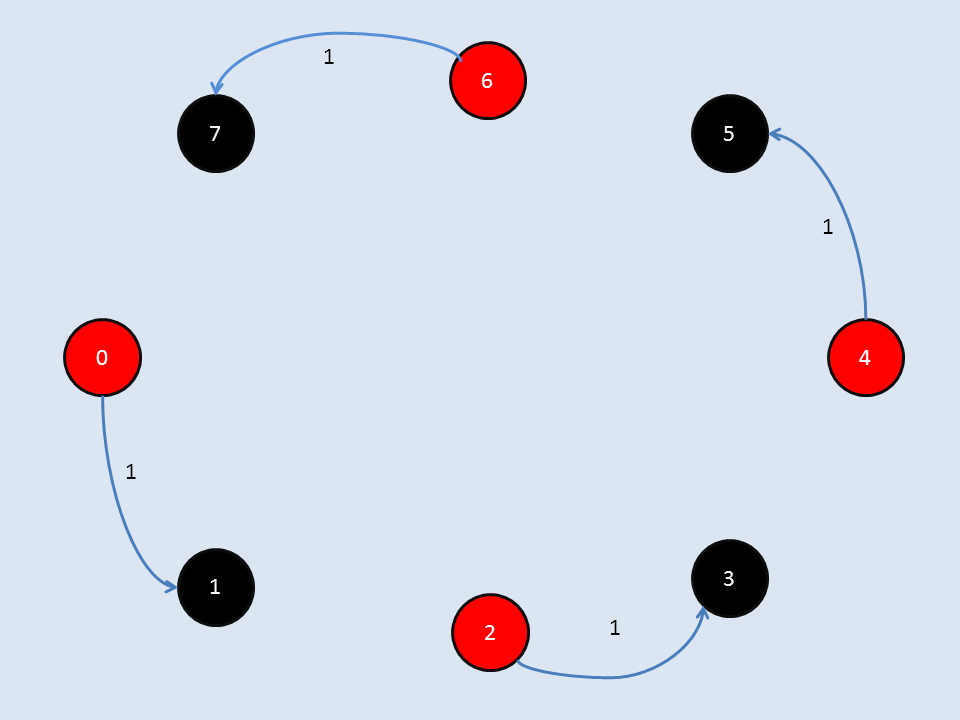
\includegraphics[scale = 0.45]{migrPari1.png}
\caption{ Primo passo di migrazione nel caso di numero pari di nodi. I numeri indicati sui nodi sono i numeri d'ordine. }
\label{fig:migrPari1}
\end{figure}

\begin{figure}[bt]
\centering
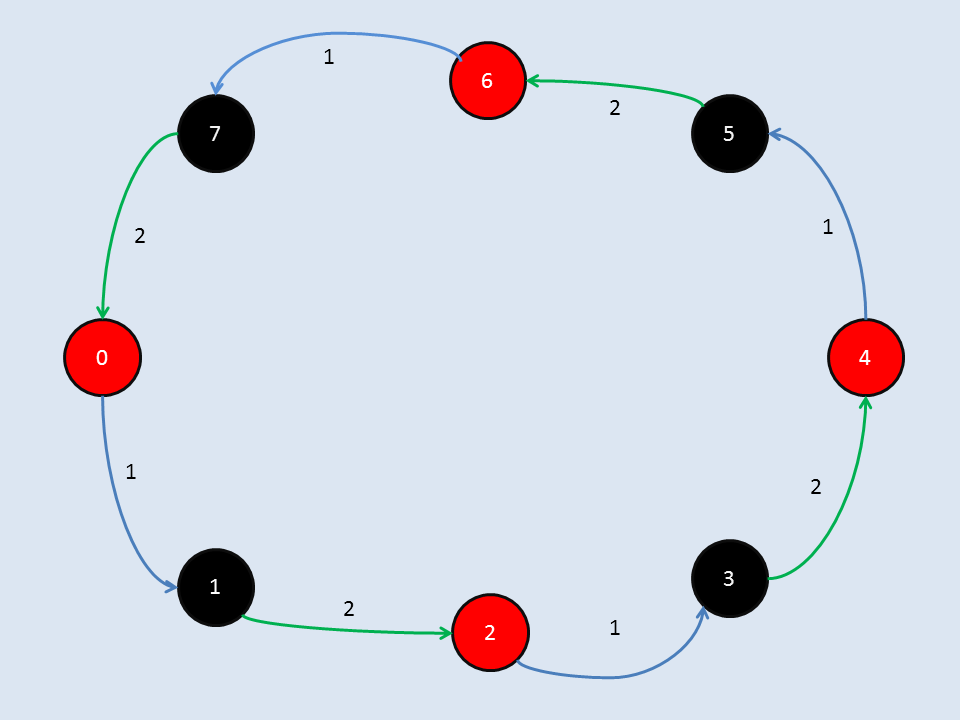
\includegraphics[scale = 0.45]{migrPari2.png}
\caption{ Secondo passo di migrazione nel caso di numero pari di nodi. I numeri indicati sui nodi sono i numeri d'ordine. }
\label{fig:migrPari2}
\end{figure}

Se invece il numero di nodi � dispari cambia solo il comportamento dell'ultimo nodo del ciclo (quello con numero d'ordine $N-1$), che sar� un nodo rosso, e del
penultimo, che sar� un nodo nero.
Durante il primo passo, infatti, l'ultimo nodo del ciclo eseguir� la \texttt{send} sul primo nodo del ciclo (anch'esso rosso), ma dovr� attendere che quest'ultimo
termini la \texttt{send} a sua volta invocata sul secondo nodo del ciclo. Il primo passo dell'ultimo nodo sar� di fatto temporalmente coincidente con il secondo
passo del primo nodo (e quindi di tutti i primi N-2 nodi). Analogamente, nel suo secondo passo, il penultimo nodo dovr� attendere che avvenga il trasferimento
tra l'ultimo nodo ed il primo, per poi effettuare il trasferimento con l'ultimo.
In altri termini, pur non cambiando nulla dal punto di vista logico, nel caso di nodi pari la fase di migrazione avviene approssimativamente nel tempo necessario
ad effettuare due trasferimenti tra nodi successivi (supponendo momentaneamente che i trasferimenti abbiano tutti lo stesso costo), mentre nel caso di nodi dispari
� necessario un tempo pari a tre trasferimenti tra nodi successivi, perch� non tutti i trasferimenti possono avvenire in parallelo.

Si noti che la scelta di uno schema di migrazione non circolare comporterebbe difficolt� nello schema delle chiamate bloccanti, con conseguente perdita di 
parallelismo delle comunicazioni (un nodo potrebbe essere costretto ad aspettare che il suo corrispondente esegua un'altra cominicazione con un nodo differente).

Nella sottosezione seguente si descriver� come scegliere un ciclo hamiltoniano \emph{bilanciato}, ossia tale che il costo per il trasferimento di un messaggio tra due
core consecutivi nel ciclo sia approssimativamente uguale per tutte le coppie di nodi consecutivi.

Nel caso dell'SCC, si assumer� come costo di trasferimento tra due core il numero di hop che separano il core ricevente dal core trasmittente, poich� tutti i
messaggi hanno la stessa dimensione. Si ricorda che il routing effettuato dalla mesh � un semplice routing x-y.


\subsection{Ricerca di cicli hamiltoniani}
La ricerca di un ciclo hamiltoniano in un grafo, in generale, � un problema intrattabile.
In questo caso, in realt�, la soluzione del problema � di per s� immediata, in quanto ogni core dell'SCC pu� comunicare con tutti gli altri core.
Si tratta di un grafo completamente connesso, e per questo motivo ogni permutazione dei nodi di calcolo � un ciclo hamiltoniano.

Ciononostante non � conveniente scegliere un ciclo in modo causale, ma conviene sfruttare la topologia e le simmetrie della mesh, cercando per quanto possibile
di far prevalere comunicazione tra nodi vicini, possibilmente all'interno dello stesso tile.

In generale, l'applicazione pu� avere a disposizione un sottoinsieme qualsiasi dei 48 core, ed � dunque necessario delineare una procedura generale per la
ricerca di un cammino hamiltoniano favorevole.

La scelta che � stata fatta per eseguire in modo relativamente semplice la ricerca � la seguente:
\begin{itemize}
	\item trattare separatamente alcuni casi particolarmente favorevoli per cui � possibile trovare la soluzione ottima in modo semplice
	\item nel caso generale utilizzare un'euristica semplice, ma che in pratica porta a risultati accettabili
\end{itemize}

Per non appesantire troppo l'implementazione, non sono stati trattati separatamente alcuni casi favorevoli leggermente pi� complicati
\footnote{Sarebbe comunque semplice estendere il lavoro per trattare anche questi casi}.

Definiamo la \emph{matrice di disponibilit�} dell'SCC come una matrice avente 8 righe e 6 colonne che ricalca la struttura della mesh. Ogni elemento
della matrice di disponibilit� corrisponde al core che nella mesh ha la stessa posizione.
Se il core in posizione $(i,j)$ nella mesh � disponibile per la computazione, allora l'elemento $(i,j)$ della matrice di disponibilit� contiene
l'identificatore (rank) di tale core. In caso contrario, l'elemento $(i,j)$ contiene l'elemento $-1$.
Gli indici di riga e colonna sono numerati a partire da $0$.
Chiameremo \emph{disponibile} un elemento della matrice $(i,j)$ se quell'elemento � maggiore di $-1$ (e quindi se il core corrispondente � disponibile
per supportare un'unit� di esecuzione dell'applicazione).

Viene fatto un primo semplice test per verificare se la matrice di disponibilit� contiene un'unica sottomatrice rettangolare (di dimensioni qualsiasi)
contenente solo elementi disponibili. Se il test ha risultato positivo, si cercano cammini ottimali, altrimenti si applica l'algoritmo generale
\footnote{Si potrebbe estendere il test a casi in cui ci sono pi� sottomatrici quadrate di soli elementi disponibili}.

L'algoritmo generale consiste nello scandire la matrice di disponibilit� per colonne nel modo indicato in figura \ref{fig:genPath}
e selezionare solamente gli elementi disponibili, aggiungendoli al cammino man mano che si incontrano.

\begin{figure}[bt]
\centering
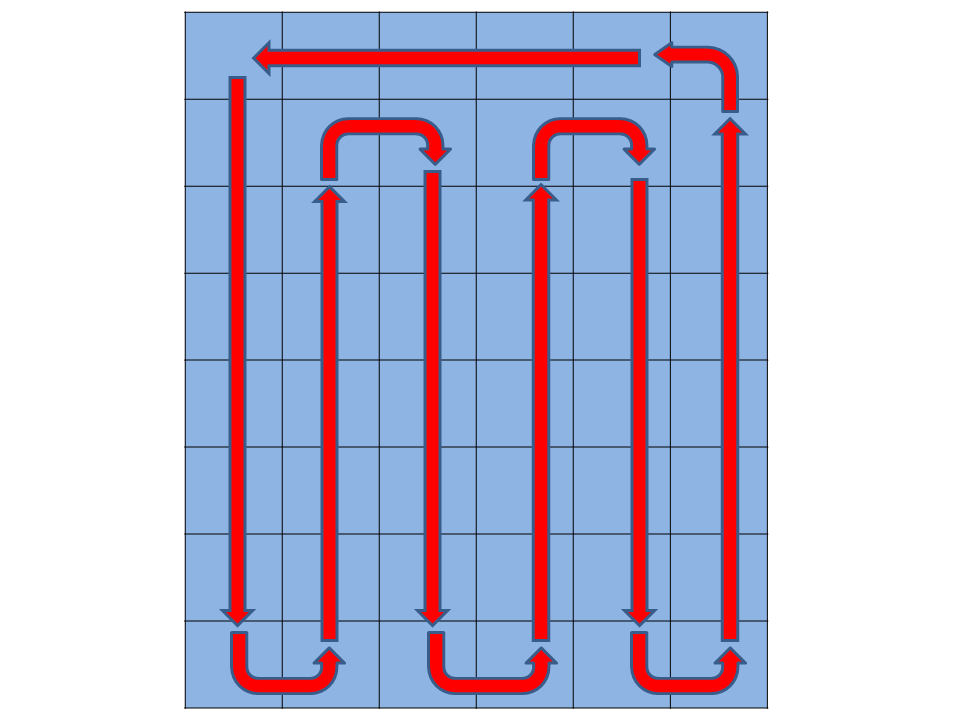
\includegraphics[scale = 0.45]{genPath.png}
\caption{ Percorso seguito dall'algoritmo generale }
\label{fig:genPath}
\end{figure}

\vspace{0.5cm}

Supponiamo ora che il test precedente abbia dato risultato positivo.
Nel caso in cui la sottomatrice individuata sia una matrice riga (colonna), la soluzione ottima, comunque poco bilanciata, prevede che l'ordine
del ciclo segua esattamente la riga (colonna) individuata.

Poniamoci adesso nel caso pi� generale in cui la sottomatrice individuata abbia un numero di righe e colonne strettamente maggiore dell'unit�.
Di stinguiamo i casi seguenti:
\begin{enumerate}
	\item Se la sottomatrice ha un numero dispari di righe ed un numero dispari di colonne, non � sempre possibile trovare un ciclo perfettamente
		  bilanciato, ma si � costretti ad accettare la presenza di un trasferimento che ha costo maggiore degli altri\footnote{Potrebbe comunque
		  verificarsi il caso favorevole in cui tale comunicazione ha lo stesso costo delle altre, in quanto effettuata tra due tiles adiacienti}. Il ciclo scelto �
		  evidenziato in figura \ref{fig:oddPath}, nel caso di una sottomatrice 5x7.
	\item Se la sottomatrice ha un numero di righe pari e maggiore di quattro, ha un numero di righe dispari, e se il pi� piccolo indice di 
		  riga corrispondente a elementi disponibili nella matrice � pari, si pu� seguire il percorso
		  indicato in figura \ref{fig:verticalTilesPath}, che ha il vantaggio di comportare solo comunicazioni intra-tile nel primo passo
		  della fase di migrazione e solo comunicazioni inter-tile (dallo stesso costo) nel secondo passo\footnote{Si osservi che in questo caso
		  il numero di nodi � pari}. Si ottiene cos� una soluzione perfettamente bilanciata.
	\item Se la sottomatrice ha un numero di righe multiplo di quattro, un numero di colonne maggiore di due, e se il pi� piccolo indice di 
		  riga corrispondente a elementi disponibili nella matrice � pari, allora si pu� seguire il percorso rappresentato in figura
		  \ref{fig:horizontalTilesPath}, che ha le stesse propriet� del ciclo scelto al punto precedente.
	\item Se non valgono i casi 2 e 3, e la sottomatrice ha un numero pari di colonne ed un numero di righe maggiore o uguale di due, �
		  possibile seguire un ciclo del tipo rappresentato in figura \ref{fig:verticalPath}.
	\item Se non valgono i casi 2 e 3, e la sottomatrice ha un numero pari di righe ed un numero di colonne maggiore o uguale di due, �
		  possibile seguire un ciclo del tipo rappresentato in figura \ref{fig:horizontalPath}.
\end{enumerate}

\begin{figure}[bt]
\centering
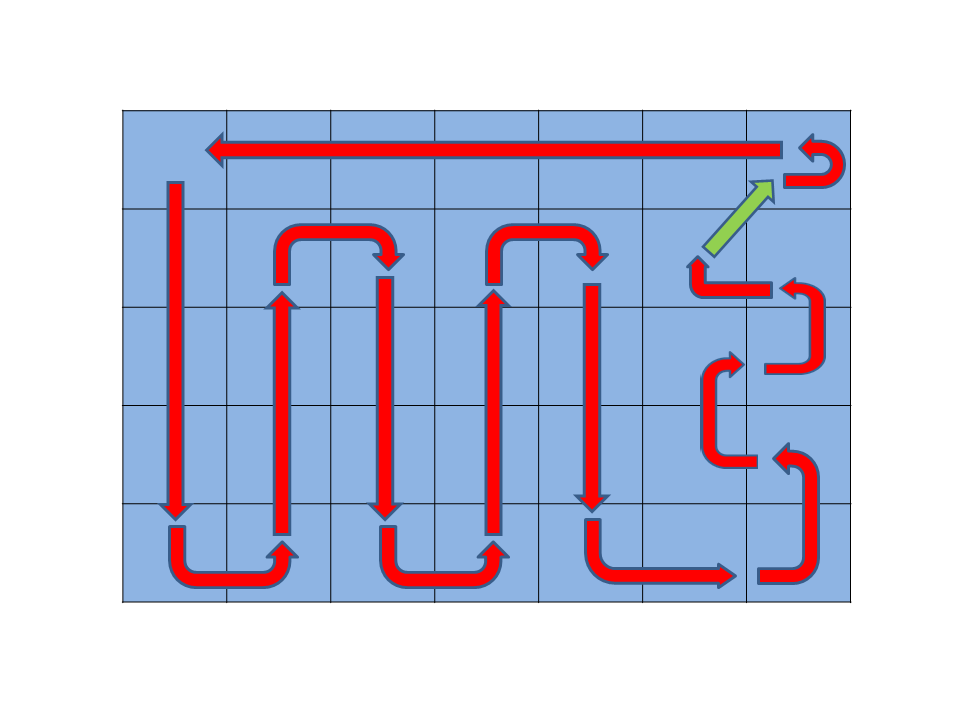
\includegraphics[scale = 0.45]{oddPath.png}
\caption{ Ciclo scelto nel caso di sottomatrice con numero dispari di elementi. In verde � evidenziata la comunicazione in generale pi� lenta rispetto alle altre. }
\label{fig:oddPath}
\end{figure}

\begin{figure}[bt]
\centering
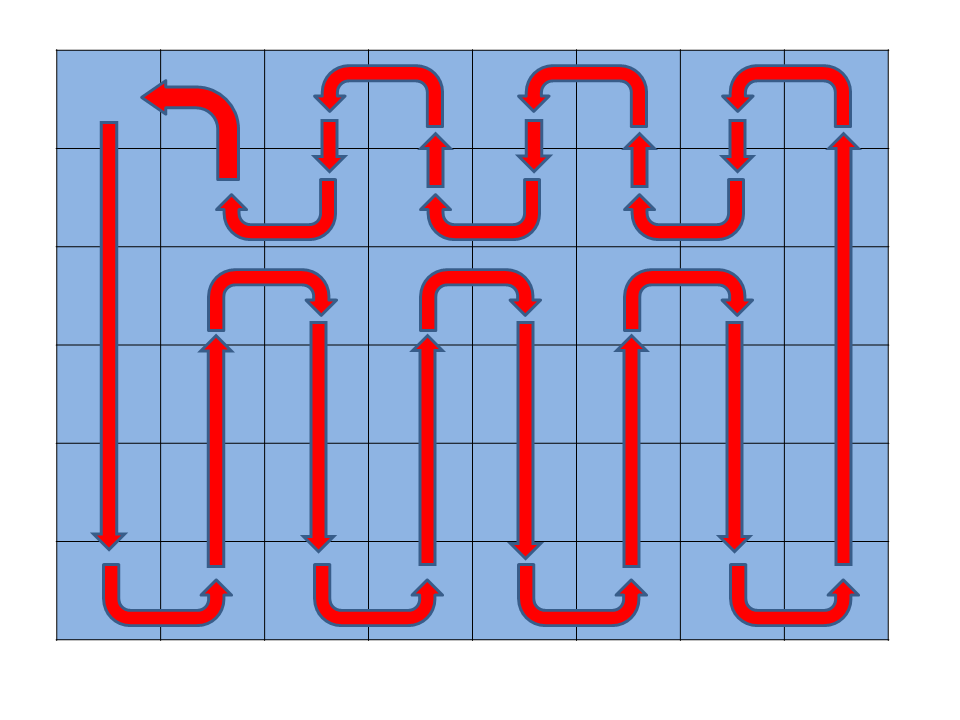
\includegraphics[scale = 0.45]{verticalTilesPath.png}
\caption{ Ciclo scelto nel caso 2 }
\label{fig:verticalTilesPath}
\end{figure}

\begin{figure}[bt]
\centering
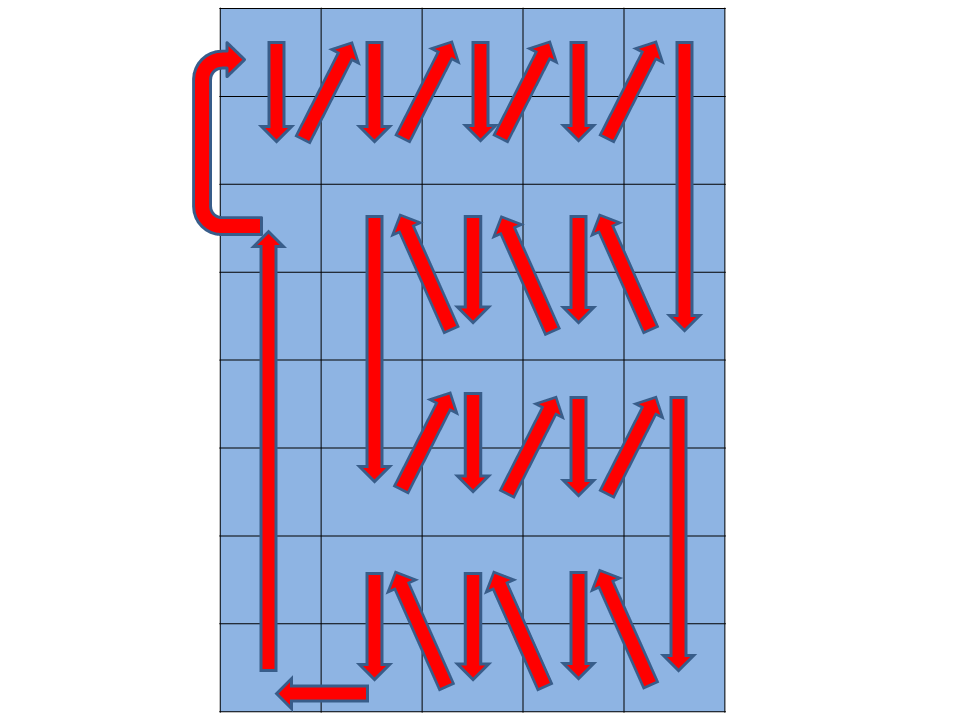
\includegraphics[scale = 0.45]{horizontalTilesPath.png}
\caption{ Ciclo scelto nel caso 3 }
\label{fig:horizontalTilesPath}
\end{figure}

\begin{figure}[bt]
\centering
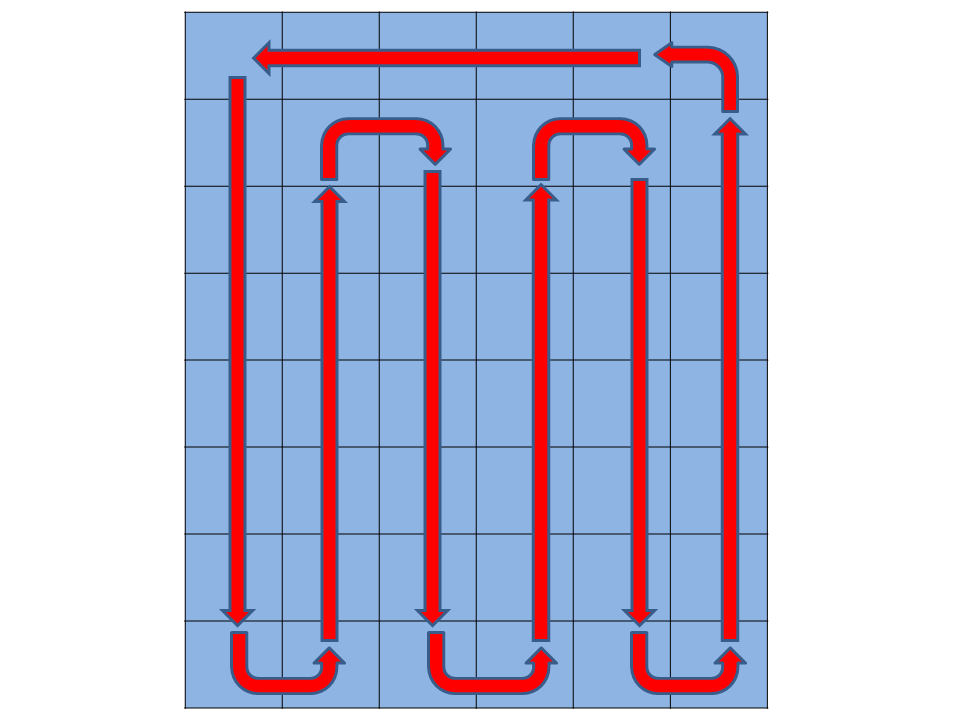
\includegraphics[scale = 0.45]{verticalPath.png}
\caption{ Ciclo scelto nel caso 4 }
\label{fig:verticalPath}
\end{figure}

\begin{figure}[bt]
\centering
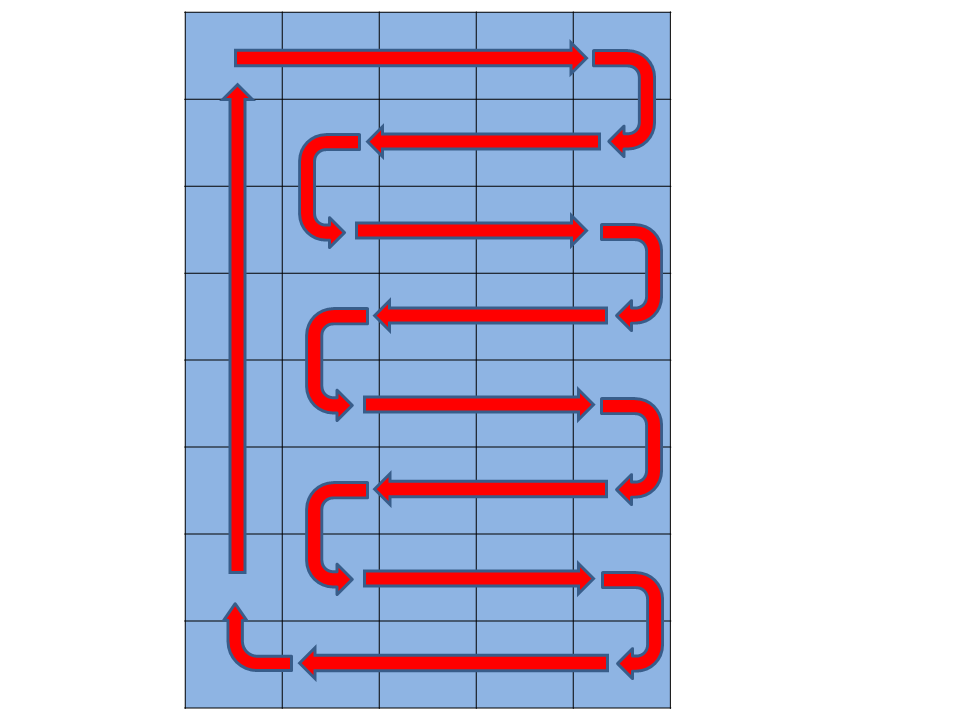
\includegraphics[scale = 0.45]{horizontalPath.png}
\caption{ Ciclo scelto nel caso 5 }
\label{fig:horizontalPath}
\end{figure}


\section{Algoritmo distribuito di terminazione}
\label{sez:term}
Come ultima questione, bisogna stabilire in che modo i nodi di calcolo devono coordinarsi per stabilire di fermare l'esecuzione prima che il numero
massimo di iterazioni sia stato raggiunto. Nel caso sequenziale, quando l'algoritmo converge ad una soluzione (ossia quando gli individui tendono ad uniformarsi
completamente), � sufficiente interrompere l'evoluzione e terminare l'esecuzione.

Nel caso parallelo, a causa della migrazione, ci sono tante popolazioni (una per ogni nodo), ed ogni nodo valuta indipendentemente dagli altri la condizione di
convergenza. Di conseguenza, i nodi possono decidere di essere arrivati a convergenza in iterazioni differenti, in modo sostanzialmente non prevedibile.

Inoltre, se un nodo decide che non ha pi� senso continuare l'evoluzione, non pu� semplicemente terminare l'esecuzione, perch� i nodi adiacenti (i quali potrebbero
non aver ancora deciso di fermarsi) effettuano delle chiamate bloccanti su di esso: si arriverebbe cos� ad una situazione di stallo. Detto in altri termini, una fase di 
migrazione deve essere eseguita da tutti i nodi oppure da nessun nodo, altrimenti si raggiunge sicuramente una situazione di stallo.

Infine, quando tutti hanno terminato, � necessario raccogliere le soluzioni locali a ciascun nodo, cosa che pu� essere fatta da un solo nodo designato appositamente.
In ogni caso, dunque � necessario che i tutti i nodi raggiungano un punto di sincronizzazione finale.

\vspace{0.5cm}

Per questi motivi, l'algoritmo di terminazione distribuita � stato concepito in maniera tale che l'evoluzione termini per tutti i nodi esattamente alla
stessa iterazione, dopo che tutti i nodi, tramite un semplice protocollo di segnalazione, abbiano deciso di comune accordo di voler terminare.

Allo scopo di non appesantire le comunicazioni, il protocollo di segnalazione agisce solamente durante le fasi di migrazione\footnote{Infatti, anche se
protocollo di segnalazione ha bisogno di trasmettere un solo byte, la trasmissione di un messaggio da un core all'altro comporta comunque un overhead
dovuto alla sincronizzazione, soprattutto a causa delle attese attive}. Pi� in dettaglio, un byte aggiuntivo
viene posto in coda al messaggio contentente il materiale genetico da propagare verso i nodi successivi. Questo byte contiene l'informazione necessaria al nodo
per decidere come agire.

I segnali si trasferiscono nel ciclo muovendosi alla velocit� di due nodi per migrazione. Infatti il nodo rosso avente numero d'ordine $i$
invia nel primo passo di una fase di migrazione un messaggio al nodo nero avente numero d'ordine $i+1$, il quale durante il secondo passo della stessa fase
di migrazione invia un altro messaggio (il cui byte di segnalazione tiene conto del messaggio appena ricevuto dal nodo $i$) al nodo rosso avente
numero d'ordine $i+2$.

\vspace{0.5cm}

Quando nessun nodo � ancora arrivato a convergenza, il byte del protocollo di segnalazione viene impostato con un segnale (\texttt{K}) che indica al nodo 
successivo di continuare tranquillamente l'evoluzione.

Quando un nodo converge, per esso comincia la prima fase dell'algoritmo di terminazione. Il nodo arrivato a convergenza segnala al nodo successivo la sua volont� di fermarsi,
inviandogli il segnale \texttt{S}, ma solamente se anche il nodo precedente gli ha a sua volta gi� inviato (in passato) tale segnale, avendo espresso la stessa volont�.
Perch� questa condizione si verifichi prima o poi per tutti i nodi, � chiaramente necessario prevedere l'esistenza di un nodo coordinatore, che non appena arrivato a convergenza
invii \texttt{S} al nodo successivo il segnale \texttt{S} senza attendere oltre. In questo modo, quando il nodo coordinatore riceve il segnale \texttt{S}, � sicuro
che tutti i nodi nel sistema sono arrivati a convergenza ed hanno deciso di essere pronti a fermarsi.

\vspace{0.5 cm}

A questo punto comincia la seconda fase dell'algoritmo, la
fase di \emph{countdown}.
Questa fase, inaugurata ancora una volta dal nodo coordinatore (l'unico che pu� essere sicuro che la decisione di terminare l'evoluzione sia stata presa
unanimemente), ha lo scopo di far terminare tutti i nodi esattamente durante la stessa iterazione, in modo tale che non possano nascere situazioni di stallo
dovute a fasi di migrazioni eseguite solo da un sottoinsieme dei nodi.

A questo scopo, il nodo coordinatore imposta un contatore locale ad un certo valore (specificato di seguito) ed invia al nodo successivo il segnale \texttt{C},
che indica l'inizio della fase di countdown. Un nodo che riceve il segnale \texttt{C} lo trasmette appena possibile al suo nodo successivo, impostando a sua volta
un contatore locale ad un certo valore.
Ad ogni fase di migrazione successiva a quella in cui � stato impostato, il contatore viene decrementato.
Il valore iniziale del contatore varia da nodo a nodo, e dipende solamente dal numero d'ordine del nodo. Questo valore deve essere calcolato in modo tale che il
contatore raggiunga il valore zero per tutti i nodi esattamente nella stessa iterazione. In questo modo, quando un nodo si accorge che il proprio contatore �
arrivato a zero, pu� terminare in tutta sicurezza l'evoluzione.

Si pu� verificare facilmente che, per il nodo avente numero d'ordine $i$ il contatore deve essere impostato al valore
\begin{equation}
	\lfloor   \frac{ 2 \lfloor \frac{N}{2} \rfloor - i }{2}  \rfloor
\end{equation}

Le figura \ref{fig:machineNormal} rappresenta in modo schematico la macchina a stati che esprime l'algoritmo di terminazione per quanto riguarda un nodo
non coordinatore.
Sugli archi che rimangono sullo stesso stato sono indicate le operazioni effettuate dal nodo quando si trova in quello stato. L'operazione \texttt{signal(X)} indica
l'invio di un segnale al nodo successivo (protocollo di segnalazione). Sugli archi che collegano due stati distinti sono presenti nomi di segnali o la variabile
di stato \texttt{readyToStop}. Un nome di segnale X indica l'evento `ho ricevuto in passato il segnale X dal mio nodo precedente`, mentre la variabile \texttt{readyToStop}
viene settata quando un nodo arriva a convergenza.

Analogamente, la figura \ref{fig:machineCoord} rappresenta la macchina a stati che esprime l'algoritmo di terminazione relativo al nodo coordinatore.

\begin{figure}[bt]
\centering
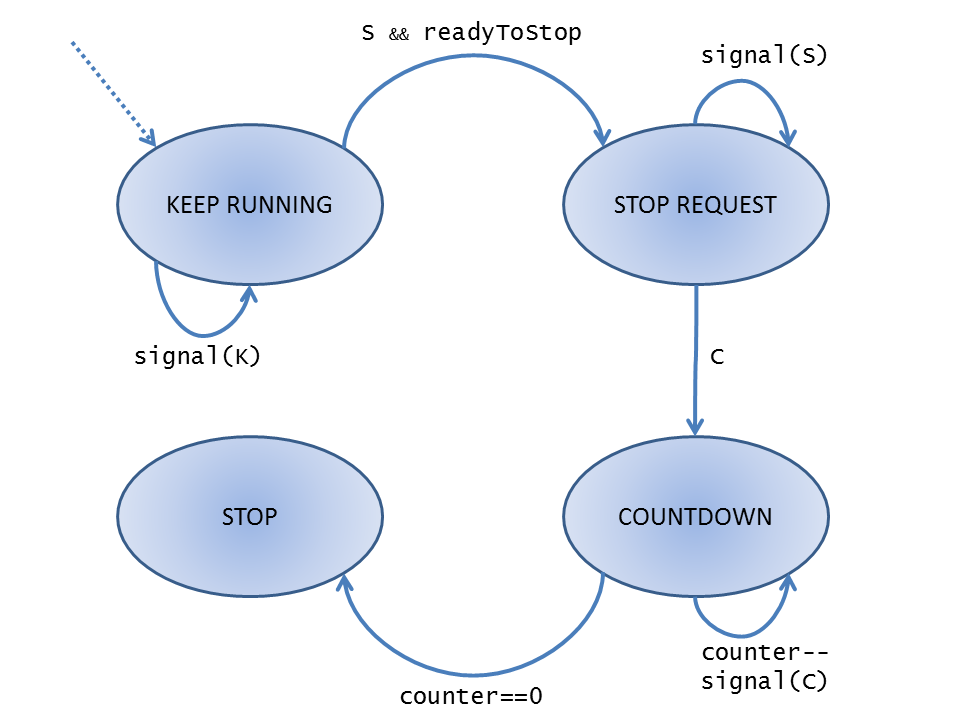
\includegraphics[scale = 0.45]{machineNormal.png}
\caption{ Macchina a stati per l'algoritmo di terminazione relativa ad un nodo non coordinatore }
\label{fig:machineNormal}
\end{figure}

\begin{figure}[bt]
\centering
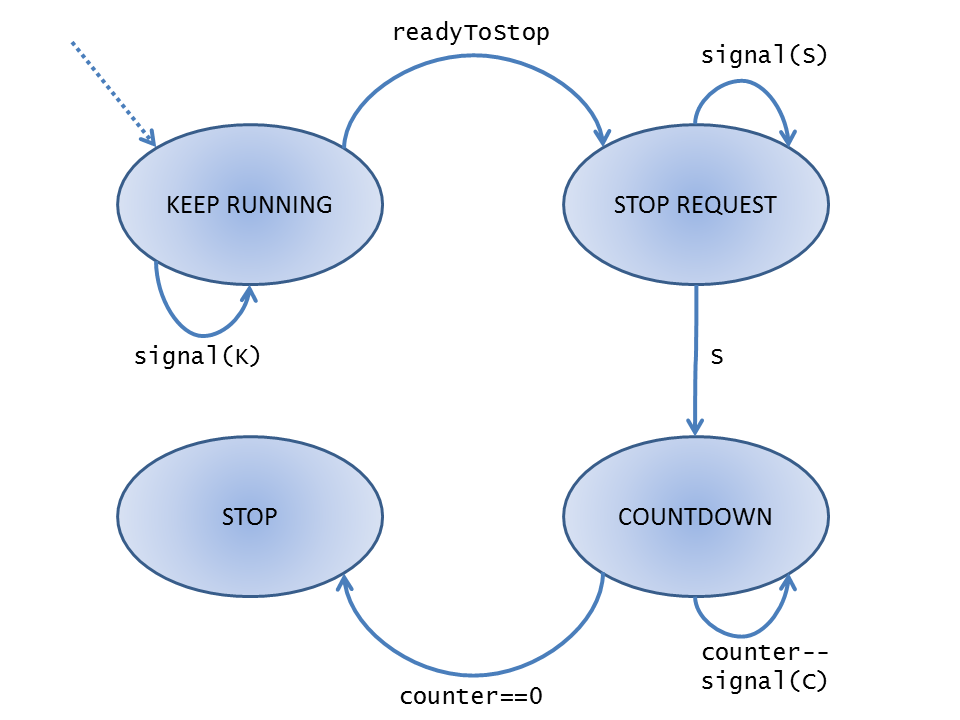
\includegraphics[scale = 0.45]{machineCoord.png}
\caption{ Macchina a stati per l'algoritmo di terminazione relativa al nodo coordinatore }
\label{fig:machineCoord}
\end{figure}


\section{Raccolta dei risultati}
\label{sez:raccolta}
Una volta terminata l'evoluzione, bisogna raccogliere i risultati. A questo scopo un nodo di calcolo viene scelto per effettuare questo compito. Per
convenzione si sceglie il nodo avente identificatore 0. Il nodo 0 invoca, in sequenza, una \texttt{receive} su ogni altro nodo. Ogni nodo con 
identificatore maggiore di zero, d'altra parte, effettua una \texttt{send} inviando al nodo 0 il suo individuo con fitness pi� alta.
In questo modo il nodo 0 pu� calcolare la soluzione globale e restituirla al chiamante (la sezione \ref{sez:interf} specifica l'interfaccia offerta dal
framework).



\chapter{Interfaccia ed implementazione}
In questo capitolo viene presentata l'interfaccia che il framework di ottimizzazione fornisce all'utente e vengono
esposti alcuni dettagli implementativi del framwork stesso.

\section{Interfaccia}
\label{sez:interf}
Il framework � stato implementato sull'SCC utilizzando la libreria RCCE. Poich� la libreria RCCE adotta il paradigma 
\emph{Single Program Multiple Data} (SPMD), anche l'utente deve attenersi allo stesso paradigma.

Ciononostante, questo non comporta praticamente nessun disagio o difficolt� per l'utente inesperto nel momento in cui egli compila
un programma che si limita ad utilizzare il framework per effettuare una qualsiasi ottimizzazione.
\'E pertanto sufficiente seguire le istruzioni riportate di seguito.

\vspace{0.5cm}

Creato un file sorgente C++ contenente la funzione \emph{main}, � necessario includere l'header `ga.h`.
Prima di creare gli oggetti necessari per impostare l'algoritmo, � necessario eseguire la chiamata di funzione
\texttt{GAUtils::frameworkInit( \&argc, \&argv )}, che inizializza il framework passando a RCCE i parametri passati
dalla linea di comando\footnote{Una volta compilato il sorgente, si deve lanciare l'eseguibile utilizzando l'utilit�
\texttt{rccerun}, il cui funzionamento � descritto in \cite{SCCprogrammers}}.

Una volta fatto questo, � necessario creare un oggetto della classe template \texttt{GeneticAlgorithm}. Il primo parametro
template (IT) specifica la classe (o il tipo primitivo) che la funzione obiettivo da minimizzare accetta in ingresso, mentre il
secondo (OT) specifica il tipo di primitivo che la funzione restituisce in uscita. Il secondo parametro pu� essere solo uno
tra \texttt{float}, \texttt{double} o \texttt{int}, in quanto la minimizzazione � mono-obiettivo (questo vincolo non impone perdita
di generalit�).
Il costruttore della classe \texttt{GeneticAlgorithm} prende in ingresso quattro parametri:
\begin{enumerate}
	\item Il puntatore alla funzione obiettivo da ottimizzare. La funzione deve restituire un oggetto di tipo \texttt{OT} e deve
		  accettare in ingresso un riferimento a costante di tipo \texttt{IT} (\texttt{const IT\&}).
	\item Il puntatore alla funzione che implementa l'operatore di mutazione. Tale funzione non ha valore di ritorno, ed accetta
	      due parametri in ingresso, il primo di tipo (\texttt{const IT\&}) ed il secondo di tipo (\texttt{IT\&}). Il primo parametro
		  si riferisce all'individuo a cui l'operatore deve essere applicato, mentre il secondo si riferisce appunto all'individuo da 
		  creare per mutazione a partire dal primo.
	\item Il puntatore alla funzione che implementa l'operatore di crossover. Tale funzione non ha valore di ritorno, ed accetta
	      tre parametri in ingresso, i primi due di tipo (\texttt{const IT\&}) ed il terzo di tipo (\texttt{IT\&}). Il primi due parametri
		  si riferiscono agli individui genitori a cui l'operatore deve essere applicato, mentre il terzo si riferisce all'individuo figlio da 
		  creare per crossover a partire dai primi due.
	\item Un valore di un tipo enumerazione che specifica l'operatore di selezione. Attualmente � implementato solo l'algoritmo \emph{Stochastic
		  Universal Sampling}, dovuto a \cite{Baker}, che si specifica con il tipo enum \texttt{GAUtils::SUS}.
\end{enumerate}

Il framework fornisce degli operatori generici gi� disponibili che possono essere utilizzati con i tipi di ingresso \texttt{float}, \texttt{double},
\texttt{FloatVector} e \texttt{DoubleVector}\footnote{I tipi \texttt{FloatVector} e \texttt{DoubleVector} sono rispettivamente di vettori di
\texttt{float} e vettori di \texttt{double}, ed hanno la stessa interfaccia della classe \texttt{vector} di STL}.

Gli operatori di mutazione gi� disponibili sono
\begin{itemize}
	\item \texttt{GAUtils::mutationGaussian} - Crea l'individuo mutante sommando all'individuo da mutare un rumore Gaussiano a media nulla ed a varianza
		  che decresce con l'aumentare del numero di iterazioni.
\end{itemize}

Gli operatori di crossover gi� disponibili sono
\begin{itemize}
	\item \texttt{GAUtils::crossoverConvex} - Crea l'individuo figlio come combinazione lineare convessa degli individui genitori. In formula,
		  seleziona un numero casuale $\beta$ compreso tra $0$ e $1$ e pone $children = \beta \cdot parent_1 + (1-\beta) \cdot parent_2$.
	\item \texttt{GAUtils::crossoverScattered} - L'i-esima componente dell'individuo figlio viene scelta causalmente tra la i-esima componente
		  del primo genitore e la i-esima componente del secondo genitore.
\end{itemize}

Per utilizzare gli operatori gi� disponibili � sufficiente specificare il valore di tipo enum riportato nei precedenti due elenchi
(i.e. \texttt{GAUtils::crossoverConvex} ) al posto del corrispondente puntatore a funzione.

Sempre per quanto riguarda i tipi suindicati, il framework fornisce infine la possibilit� di generare popolazioni iniziali in modo casuale.
Per i tipi \texttt{float} e \texttt{double} � possibile invocare, sull'oggetto creato precedentemente, la funzione
\texttt{G.gaUtils.generate( population\_size, initial\_population, lower\_bound, upper\_bound )}, che accetta in ingresso un intero che indica la dimensione 
della popolazione da creare, un \texttt{vector<IT>} in cui verr� costruita la popolazione iniziale ed infine due float che specificano rispettivamente
il limite inferiore ed il limite superiore dell'intervallo monodimensionale a cui gli individui generati devono appartenere.

In modo analogo per i tipi \texttt{FloatVector} e \texttt{DoubleVector} � possibile invocare la funzione
\texttt{G.gaUtils.generate( population\_size, initial\_population, lower\_bounds, upper\_bounds )}, che accetta in ingresso un intero che indica la dimensione 
della popolazione da creare, un \texttt{vector<IT>} in cui verr� costruita la popolazione iniziale ed infine due \texttt{vector<float>} che specificano
rispettivamente i limiti inferiori ei superiori dell'intervallo multidimensionale a cui gli individui generati devono appartenere.

\vspace{0.5cm}

A questo punto � possibile invocare sull'oggetto algoritmo genetico il metodo \texttt{run} che lancia l'algoritmo genetico stesso. Questa funzione ritorna
un valore di tipo \texttt{IT}, che � la soluzione trovata dall'algoritmo. Poich� il framework va utilizzato secondo il paradigma SPMD, in realt� ogni core esegue una
sua chiamata alla funzione \texttt{run}, e ritorna un proprio valore. Come specificato nella sezione \ref{sez:raccolta}, il nodo con identificatore 0 raccoglie i
risultati e dunque e proprio quest'ultimo che ritorna la soluzione globale. Gli altri nodi ritornano la loro soluzione locale (che in genere non interessa).
Per questo motivo la classe \texttt{GeneticAlgorithm} dispone di una funzione \texttt{IamMaster()} che ritorna il valore booleano \texttt{true} quando chiamata
sul core avente identificatore 0. In questo modo l'utente pu� correttamente selezionare la soluzione globale.

La funzione \texttt{run} accetta in ingresso i seguenti parametri
\begin{enumerate}
	\item Un riferimento ad una costante di tipo vector<IT>, che specifica la popolazione iniziale da cui l'algoritmo genetico parte.
	\item Un intero che indica il massimo numero di iterazioni che possono essere eseguite prima di terminare. Valore di default = 100.
	\item Un float compreso tra 0.0 ed 1.0 che specifica la frazione di crossover (\emph{crossover fraction}). Valore di default = 0.8.
	\item Un intero positivo che specifica il numero di elite children. Valore di default = 3.
	\item Un float compreso tra 0.0 ed 1.0 che specifica la frazione di individui della popolazione corrente che vengono propagati da
		  ogni nodo verso il suo successivo durante una fase di migrazione. Valore di default = 0.1.
	\item Un intero positivo che specifica il periodo di migrazione, ossia il numero di iterazioni che intercorrono tra due fasi di migrazione successive.
\end{enumerate}

Poich� i metodi della classe \texttt{GeneticAlgorithm} possono sollevare eccezioni di tipo \texttt{GAError}, � necessario utilizzare il costrutto \texttt{try-catch}.


\section{Implementazione}
Come gi� accennato in precedenza, il framework � stato implementato facendo uso dei template C++, per permettere all'utente di effettuare minimizzazioni
di funzioni obiettivo il cui ingresso � qualsiasi.

Lavorando con i template, non potendo contare sulla keyword C++ \texttt{export}, il framework � quasi completamente contenuto in due header file,
il file `ga.h` (incluso dall'utente) ed il file `gaUtils.h`.
Il primo include il secondo, e contiene la definizione della classe \texttt{GeneticAlgorithm} (la classe principale) e quindi implementa il cuore dell'algoritmo.
Nell'header `ga.h` sono implementate anche le macchine a stati relative all'algoritmo distribuito di terminazione. Per motivi legati all'implementazione
� stato necessario creare due versioni di macchine a stati differenti per nodi di colore diverso, oltre alla differenza che esiste tra il nodo coordinatore
e gli altri nodi.
Il secondo header contiene le definizioni degli operatori genetici gi� disponibili e le funzioni per generare le popolazioni iniziali, per i quattro tipi indicati
nella sezione precedente.

Per generare numeri random con con distribuzione uniforme e gaussiana sono state usate delle librerie liberamente scaricabili sul sito
http://www.agner.org/. Il modulo per la generazione di numeri random con distribuzione uniforme � disponibile come libreria statica (`randomaelf32.a`), 
mentre il modulo che genera numeri con distribuzioni non uniforme (utilizzando la libreria statica precedente) � disponbile come sorgente C++ (`stoc1.cpp`).

Un aspetto importante del progetto � l'indipendenza del framework dalla libreria usata per la comunicazione (in questo caso RCCE), e quindi dall'intera
architettura (in questo caso SCC).
La libreria per la comunicazione � infatti racchiusa nel modulo `mesh2D`, separato dal resto del framework. Questo modulo pu� avere bisogno 
di essere inizializzato (� il caso di RCCE), ma non lascia trasparire all'esterno il modo in cui questo avviene.
Il suo scopo � sostanzialmente quello di fornire alla classe principale un'interfaccia che permette di trasmettere/ricevere ad/da un altro nodo, specificandone
l'identificatore, un certo insieme di byte (senza interpretarli). Inoltre deve effettuare il calcolo del ciclo hamiltoniano\footnote{Il calcolo dipende 
in generale dall'architettura} e dunque restituire al nodo chiamante i suoi parametri di configurazione nella mesh: il suo identificatore, il suo numero
d'ordine, il suo colore, l'identificatore del nodo che lo precede nel ciclo, l'identificatore del nodo che ad esso segue. Note queste informazioni,
l'algoritmo genetico parallelo descritto nel capitolo precedente ha tutto ci� che occorre per il funzionamento.

Come conseguenza diretta dell'indipendenza da architettura e libreria, � possibile, cambiando l'implementazione del modulo `mesh2D`, far girare l'algoritmo
su una tradizionale rete di calcolatori, ad esempio attraverso l'uso dei socket. Ovviamente in quest'ultimo caso pu� diventare problematica la ricerca di un
ciclo hamiltoniano sufficienetemente bilanciato, a meno che esso non venga impostato staticamente, cosa che pu� avvenire ad esempio in un cluster di calcolatori
connessi via LAN ad alta velocit�.

\vspace{0.5cm}

Il core dell'algoritmo utilizza due array di oggetti di tipo \texttt{IT}. Il primo array contiene la popolazione corrente\footnote{All'inizio dell'algoritmo
viene inizializzato con la popolazione iniziale passata dall'utente}, mentre il secondo viene gradualmente costruito durante l'iterazione attraverso l'applicazione
degli operatori genetici agli individui contenuti nel primo array. Alla fine dell'iterazione i due array vengono scambiati con un semplice scambio di
puntatori.

Per diversi motivi � necessario ordinare gli individui per fitness ad ogni iterazione. Ad esempio durante la selezione bisogna associare agli individui che
hanno una migliore fitness una pi� alta probabilit� di riprodursi (per mutazione o ricombinazione). Nelle fasi di migrazioni, inoltre, bisogna trasmettere al nodo
successivo gli individui con la fitness pi� altra.

A questo scopo � stato implementato un heap binario di massimo\footnote{Anche se la funzione viene minimizzata, si utilizza un heap di massimo a causa
del fitness scaling, che mappa gli individui con fitness pi� bassa in valori scalati maggiori, in modo che l'individuo migliore si trovi ad avere
il valore di fitness scalato pi� grande di tutti e cos� via}, che in ogni iterazione viene riempito con un inserimento alla volta dagli individui della
popolazione corrente (man mano che viene calcolata la loro fitness), e che viene svuotato in modo brusco alla fine dell'iterazione, in modo da poter essere
riempito nuovamente alla iterazione successiva.




\chapter{Risultati sperimentali}
Allo scopo di testare il funzionamento dell'algoritmo e verificare i vantaggi dell'elaborazione parallela, sono stati effettuati alcuni test su un problema di ottimizzazione che richiede una notevole quantit� di calcoli.

Il problema scelto consiste nell'addestramento una rete neurale feed-forward a due strati con un ingresso, quattro neuroni nascosti ed una uscita. La funzione di attivazione dei neuroni nello strato nascosto � di tipo sigmoidale, mentre quella dell'unico neurone nello strato di uscita � lineare.

I dataset scelti sono costituiti da 50 elementi. Ai fini dell'ottimizzazione, i dataset sono stati mappati linearmente sull'intervallo [-1,1]. La funzione obiettivo da minimizzare � la deviazione standard dell'errore di approssimazione sugli elementi del dataset.

\vspace{0.5cm}

Nei test effettuati sono stati utilizzate popolazioni di dimensione variabile tra 15 e 200, utilizzando un numero di core progressivamente crescente.
La popolazioni iniziali sono state inizializzate in modo casuale scegliendo i valori reali in un intervallo simmetrico centrato nell'origine.

Per quanto riguarda gli altri parametri dell'algoritmo genetico, i valori scelti sono riportati nella tabella di figura \ref{fig:tabpar}.

\begin{figure}[bt]
\centering
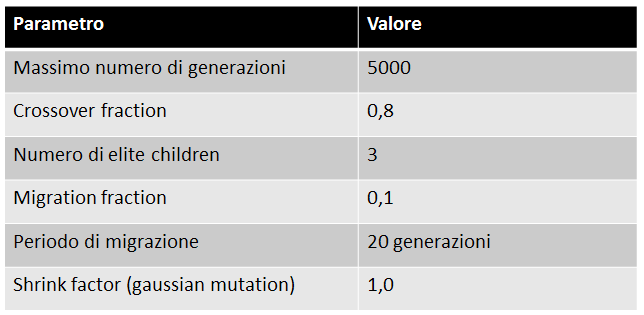
\includegraphics[scale = 0.65]{tabpar.png}
\caption{ Parametri dell'algoritmo genetico utilizzati. }
\label{fig:tabpar}
\end{figure}



\section{Dataset 1}
Il primo dataset su cui � stata effettuata l'ottimizzazione � riportato in figura \ref{fig:d1} (in cui i punti del dataset sono stati congiunti con delle spezzate).

\begin{figure}[bt]
\centering
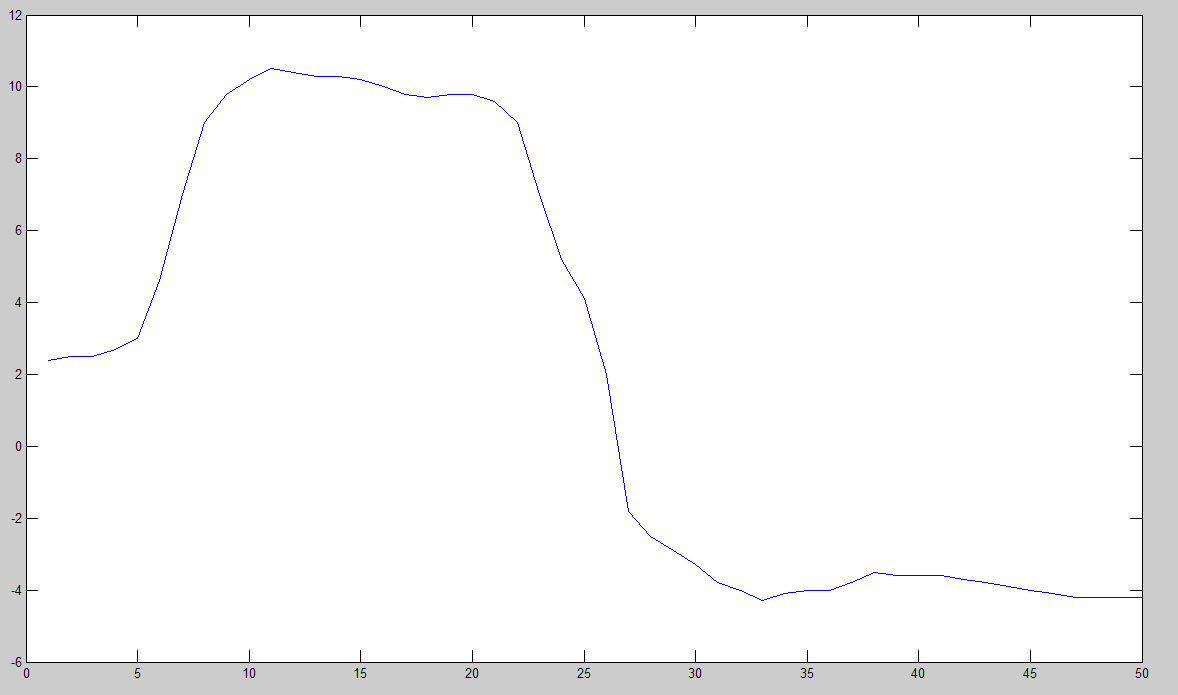
\includegraphics[scale = 0.35]{dataset1.png}
\caption{ Dataset 1 }
\label{fig:d1}
\end{figure}

I risultati ottenuti sono mostrati nella tabella di figura \ref{fig:ris1}.

Gli individui delle popolazioni iniziali sono stati inizializzati casualmente con valori appartenenti all'intervallo [-10,10].


Il grafico in figura \ref{fig:g1} mostra l'andamento dell'errore al crescere del numero di core nel caso in cui la popolazione iniziale su ciascuno core sia costituita da 20 elementi. Come � possibile notare, all'aumentare del numero di core impiegati il risultato ottenuto migliora.

\begin{figure}[bt]
\centering
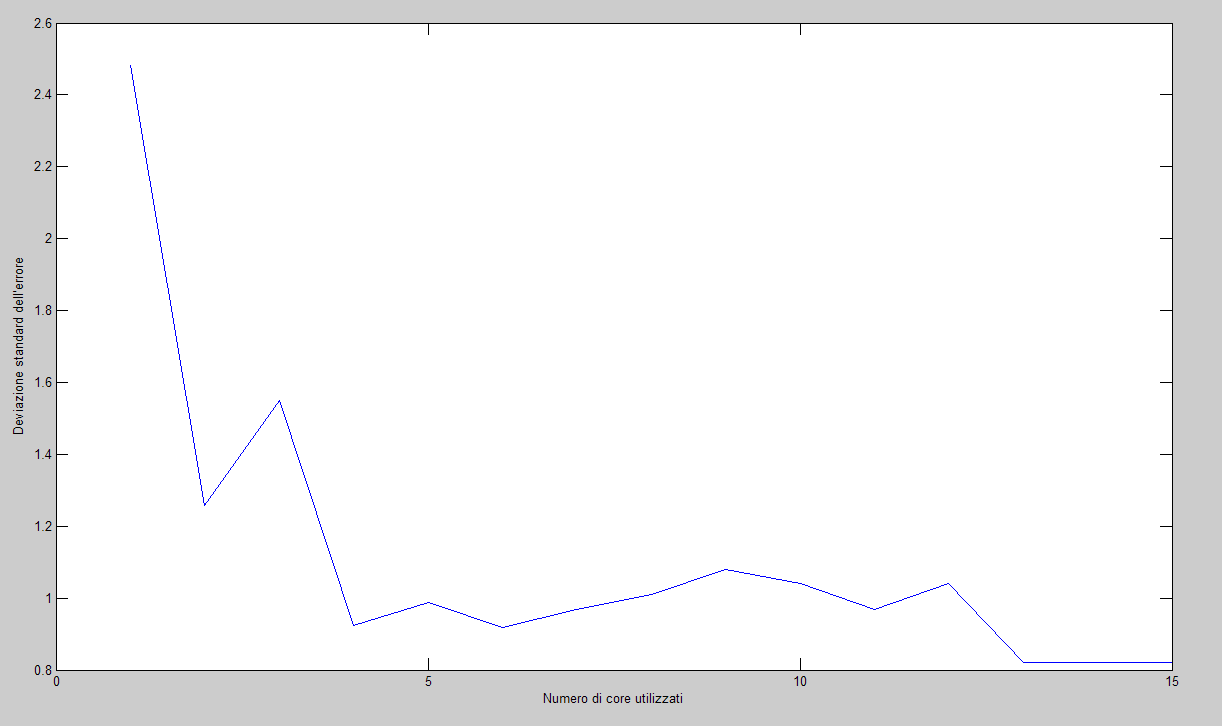
\includegraphics[scale = 0.35]{grafico1.png}
\caption{ Andamento del minimo ottenuto in funzione del numero di core impiegati per il dataset 1 }
\label{fig:g1}
\end{figure}

\begin{figure}[bt]
\centering
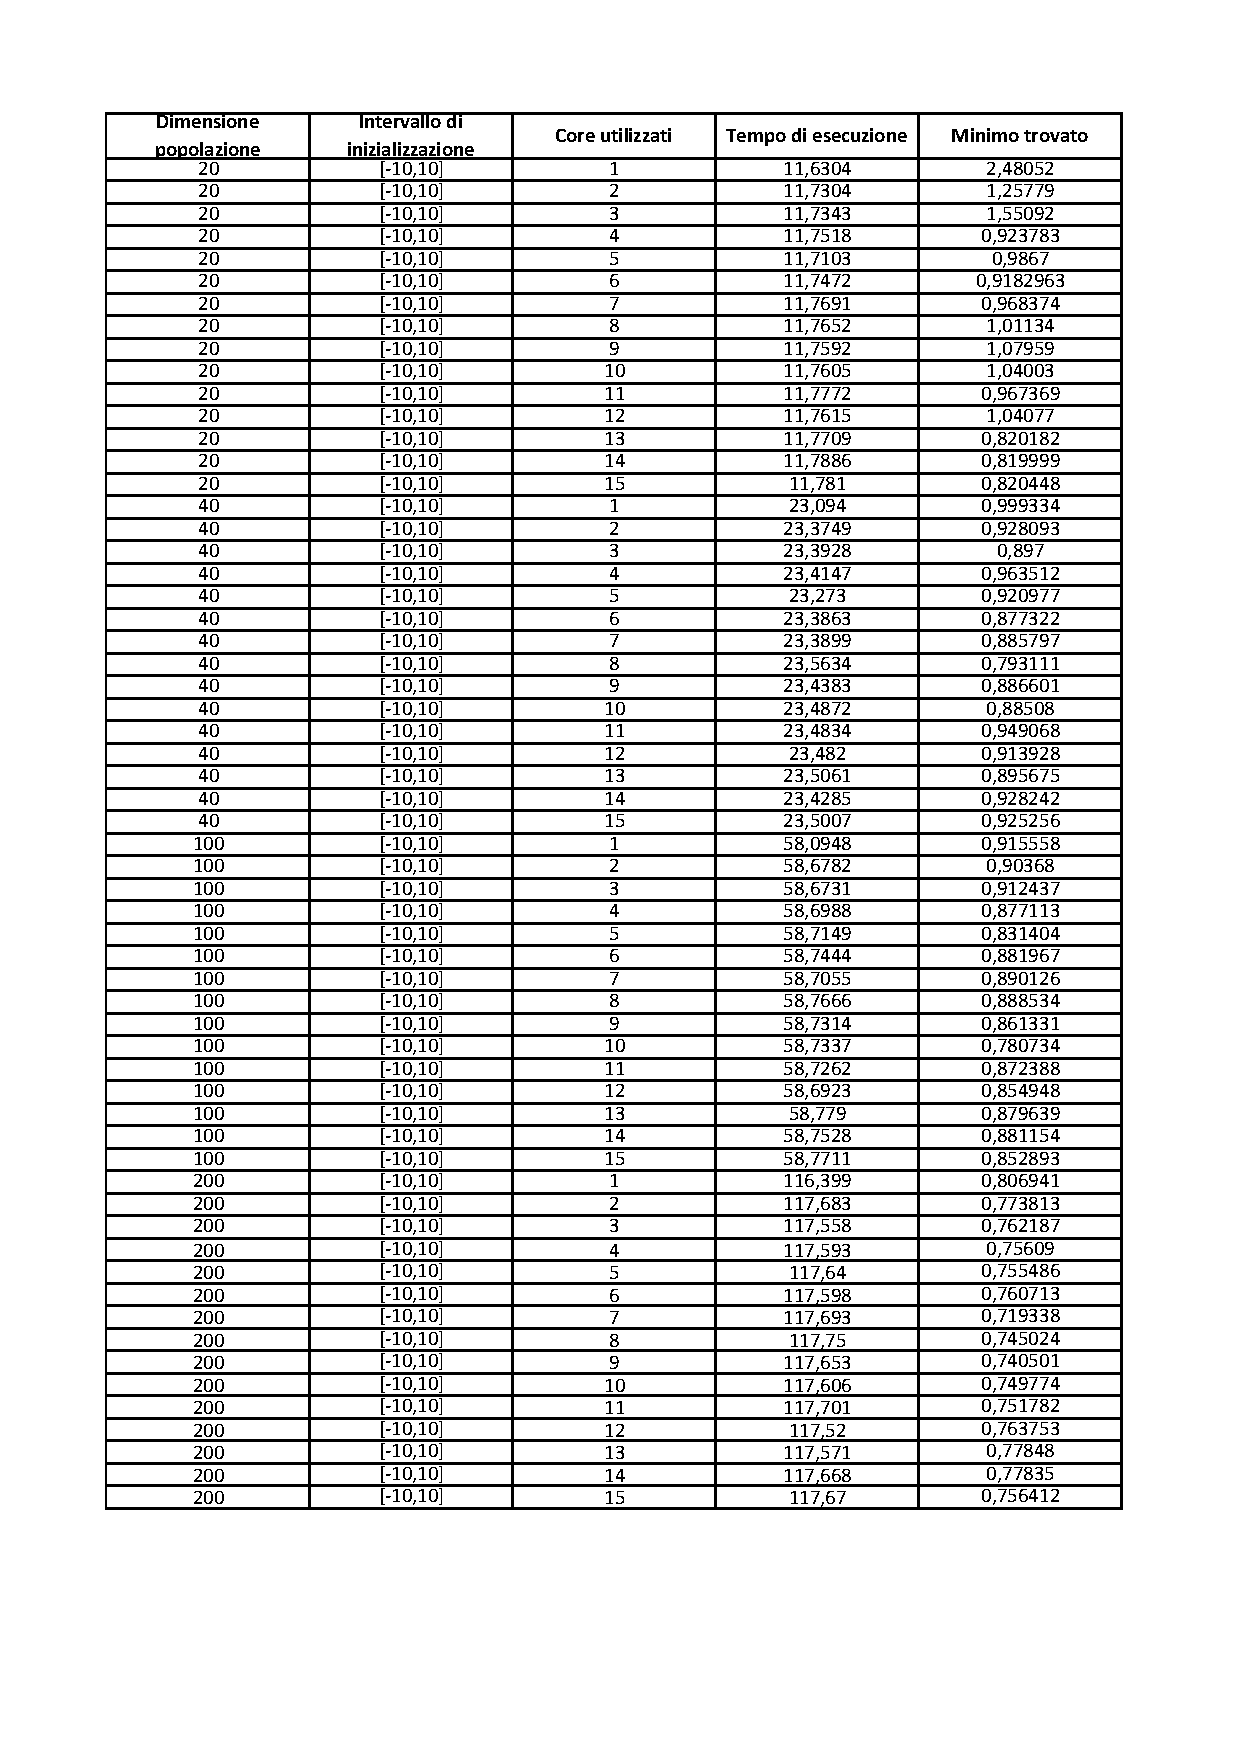
\includegraphics[scale = 0.65]{tab1.pdf}
\caption{ Tabella dei risultati per il dataset 1 }
\label{fig:ris1}
\end{figure}




\section{Dataset 2}
Il secondo dataset su cui � stata effettuata l'ottimizzazione � riportato in figura \ref{fig:d2} (in cui i punti del dataset sono stati congiunti con delle spezzate).

\begin{figure}[bt]
\centering
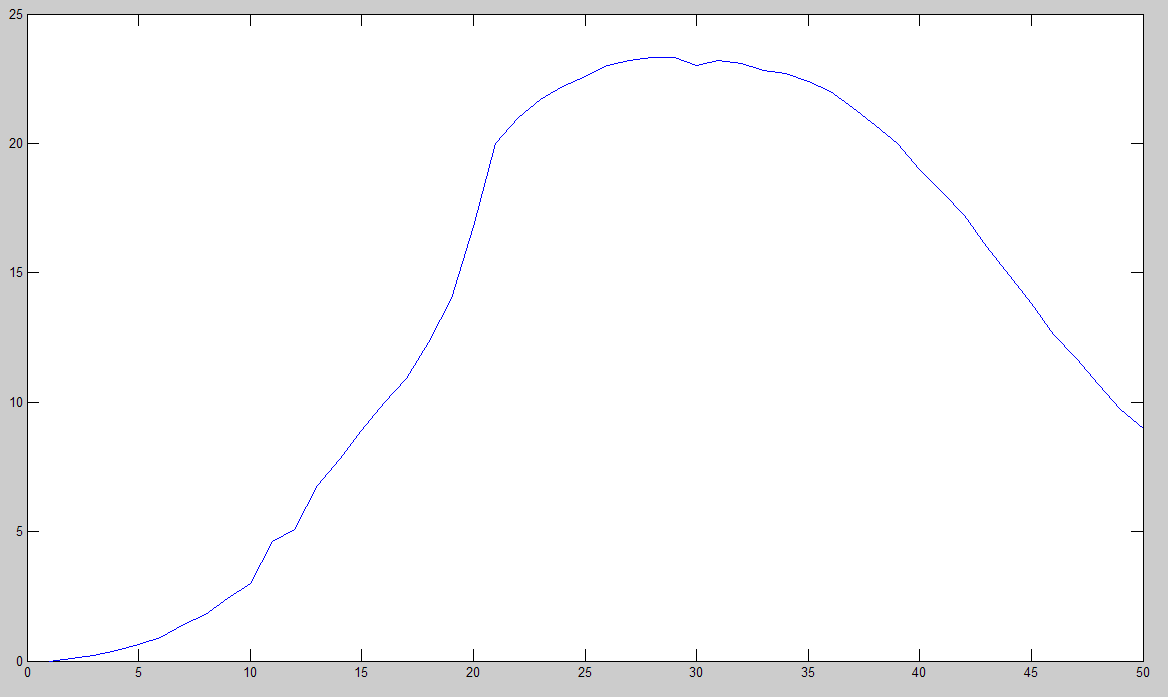
\includegraphics[scale = 0.35]{dataset2.png}
\caption{ Dataset 2 }
\label{fig:d2}
\end{figure}

I risultati ottenuti sono mostrati nella tabella di figura \ref{fig:ris2}.
In questo caso l'intervallo su cui sono stati generati casualmente gli individui delle popolazioni iniziali � stato fatto variare in funzione della dimensione della popolazione.

Il grafico in figura \ref{fig:g2} mostra l'andamento dell'errore al crescere del numero di core nel caso in cui la popolazione iniziale su ciascun core sia costituita da 80 elementi. Come � possibile notare, all'aumentare del numero di core impiegati il risultato ottenuto migliora.

\begin{figure}[bt]
\centering
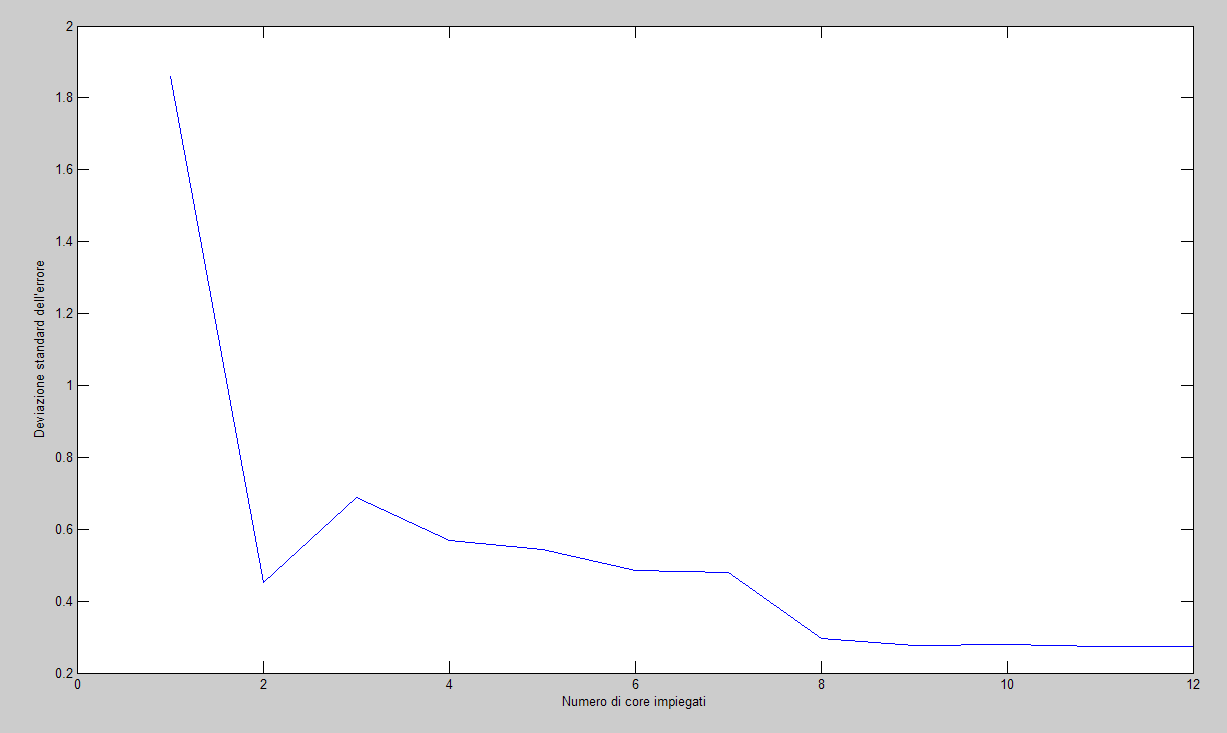
\includegraphics[scale = 0.35]{grafico2.png}
\caption{ Andamento del minimo ottenuto in funzione del numero di core impiegati per il dataset 2 }
\label{fig:g2}
\end{figure}

\begin{figure}[bt]
\centering
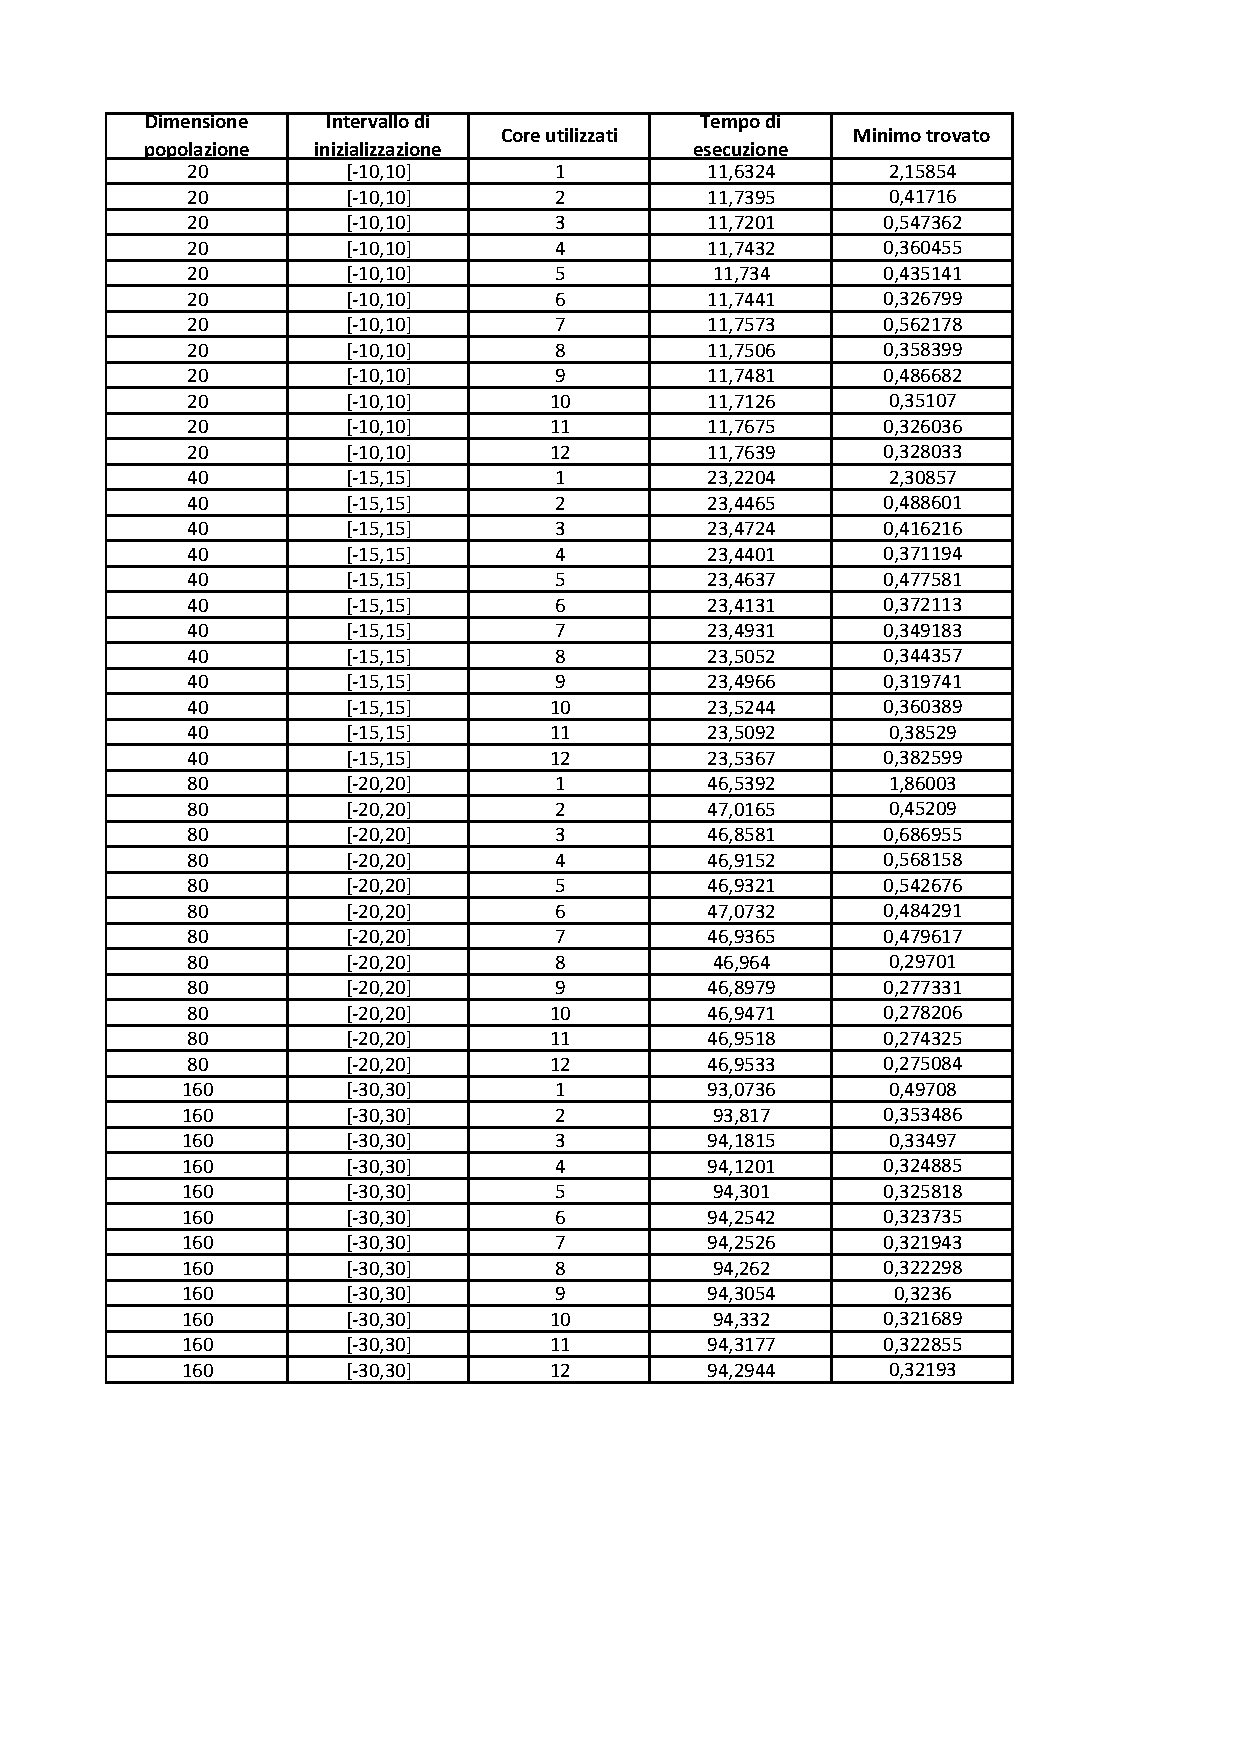
\includegraphics[scale = 0.65]{tab3.pdf}
\caption{ Tabella dei risultati per il dataset 2 }
\label{fig:ris2}
\end{figure}


\section{Considerazioni sui risultati ottenuti}
Prima di commentare i risultati, � necessario fare una osservazione. Il numero di iterazioni necessarie all'algoritmo genetico per convergere (su ciascun core) dipende molto poco dal numero di core impiegati. Questo perch� le perturbazioni casuali tramite le quali l'ottimizazione stocastica ha luogo sono dovute principalmente all'operatore di mutazione gaussiano. Questo operatore, il cui funzionamento � descritto nella sezione \ref{sec:Mutazione}, � stato definito in modo da far convergere l'algoritmo in un numero di iterazioni il cui ordine di grandezza � tendenzialmente lo stesso di quello del numero massimo di iterazioni specificato.

Solitamente il numero effettivo di iterazioni necessarie per arrivare a convergenza � inferiore al numero massimo di generazioni, perch� l'algoritmo genetico tende ad attestarsi su uno o pi� minimi locali, nel momento in cui riesce a trovarne.

Il tempo di esecuzione � dunque praticamente indipendente dal numero di core impiegati, e dipende sostanzialmente dalla dimensione della popolazione iniziale, come � possibile evincere dalle tabelle.

\vspace{0.5 cm}

Il vantaggio di avere pi� unit� di calcolo sta nella possibilit� di esplorare un dominio di ricerca pi� ampio, e dunque nella possibilit� di trovare un numero di minimi locali maggiore. Perch� questo sia possibile, bisogna inizializzare le popolazioni iniziali scegliendo valori in intervalli di inizializzazione adaguatamente dimensionati.

Questi intervalli non devono esere troppo piccoli, altrimenti si rischia che tutti i core tendano a trovare gli stessi minimi locali, rendendo di fatto completamente inutile l'impiego di tanti core\footnote{In pratica core diversi tenderebbero a fare lo stesso lavoro.}.

Allo stesso modo gli intervalli non possono essere troppo grandi, perch� altrimenti la probabilit� di trovare buone soluzioni (in relazione al minimo globale, che nel caso in esame esiste) diminuisce notevolmente. Ci� accade perch� se tutti gli individui dell'algoritmo genetico si trovano in una zona di $\mathds{R}^n$ in cui la funzione obiettivo � sostanzialmente piatta, � molto difficile l'algoritmo riesca a trovare un minimo (si procederebbe sostanzialmente per ricerca casuale).
Naturalmente bisogna tenere in considerazione che scegliendo intervalli pi� grandi � possibile trovare soluzioni migliori poich� si allarga il dominio di ricerca.

\vspace{0.5 cm}

Avendo pi� core a disposizione, in ogni caso, aumenta la probabilit� di riuscire a trovare dei minimi locali.

Di conseguenza, � possibile compensare la diminuzione della probabilit� di trovare buone soluzioni dovuta all'allargamento degli intervalli di inizializzazione con l'aumento del numero di core impegati.

\vspace{0.5 cm}

Gli esperimenti condotti sul secondo dataset mostrano come un buon compromesso tra numero di core e dimensione degli intervalli di inizializzazione porti ad un buon risultato (si veda la figura \ref{fig:g2}).

\vspace{0.5 cm}

Come ultima considerazione, si pu� notare dalle tabelle come l'impiego di popolazioni pi� numerose porti in media a risultati migliori.



\begin{thebibliography}{1}

\bibitem{tassonomia}
Riccardo Poli, Mariusz Nowostawski (1999) \\
Parallel Genetic Algorithm Taxonomy

\bibitem{microprocessorReport}
Max Baron (2010) \\
The Single-chip Cloud Computer \\
Microprocessor report, www.MPRonline.com

\bibitem{intelDeveloperManual}
Intel (1995)
Pentium� Processor Family Developer's Manual, Architecture and Programming Manual

\bibitem{intelTechnicalReport}
Howard, Dighe et al. (2010) \\
A 48-Core IA-32 Message-Passing Processor with DVFS in 45nm CMOS

\bibitem{RCCEspecification}
Tim Mattson, Rob van der Wijngaart (2010) \\
RCCE: a Small Library for Many-Core Communication - Specification document

\bibitem{RCCEpaper}
Rob van der Wijngaart, Timothy Mattson, Werner Haas (2010) \\
Light-weight Communications on Intel's Single-Chip Cloud Computer Processor

\bibitem{SCCEAS}
Intel labs (2010) \\
SCC External Architecture Specification (EAS), Revision 1.1

\bibitem{SCCprogrammers}
Intel labs (2010) \\
The SCC Programmer's Guide, Revision 0.75

\bibitem{Baker}
Baker, James E. (1987)
Reducing Bias and Inefficiency in the Selection Algorithm
Proceedings of the Second International Conference on Genetic Algorithms and their Application (Hillsdale, New Jersey: L. Erlbaum Associates)

\end{thebibliography}


\end{document}

